\documentclass[article]{elsarticle}
\usepackage{natbib}
\biboptions{numbers,sort&compress}
\usepackage{geometry}
\usepackage{setspace}
\usepackage{amssymb}
\usepackage{subfigure}
\usepackage{graphicx, xcolor}
\graphicspath{{./figures/}}
\usepackage{amsmath}
\usepackage{tabularx}
\usepackage{caption}
\usepackage{longtable}
\def\eg{{e.g.\ }}
\def\etc{{etc.\ }}
\def\etal{\mbox{\it et al.\ }}
\def\dd{\textrm{d}}
\def\ln{\textrm{ln}}
\renewcommand*{\thesubfigure}{}
%------------------------------------------------------------------------------------------%
\begin{document}
%------------------------------------------------------------------------------------------%
\begin{frontmatter}
\title{Computational Thermodynamics of the CoNiGa High Temperature Shape Memory Alloy system}
\author{Arpita Chari$^{a}$}
\author{Ebubekir Dogan$^{a}$}
\author{Anjana Talapatra$^{a}$}
\author{Avinash.R.Chivukula$^{a}$}
\author{Andres Garay$^{c}$}
\author{I. Karaman$^{a,b}$}
\author{R. Arr\'{o}yave $^{a,b,}$\fnref{label22}}
\address{$^a$ Department of Mechanical Engineering, Texas A\&M University, USA, 77843}%
\address{$^b$ Department of Materials Science and Engineering, Texas A\&M University, USA, 77843}%
\address{$^c$ Centro de Investigaci\'{o}n de Materiales Avanzados (CIMAV),Monterrey, Nuevo L\'{e}on, M\'{e}xico,}%
\fntext[label22]{Corresponding author. E-mail: rarroyave@tamu.edu}  %%
%------------------------------------------------------------------------------------------%
\begin{abstract}
The CoNiGa ternary system has recently emerged as a promising alternative to currently used high temperature Shape Memory Alloys (SMA), with possible applications in the aerospace and automotive industries. In this work, we use thermodynamic modeling based on the CALPHAD approach to investigate the thermodynamic properties, phase stability and shape memory properties of these alloys. The thermodynamic model parameters have been obtained by fitting experimental and ab initio data. The stability of the $\beta$ phase at high temperatures was enforced accurately by remodeling the CoGa system. Also, the phase stabilities of Ni$_{5}$Ga$_{3}$ ($\delta$) and Ni$_{13}$Ga$_{9}$ ($\epsilon$) were determined as they are known to cause detrimental effects in the ternary at low temperatures.
\end{abstract}
%------------------------------------------------------------------------------------------%
\begin{keyword}
CALPHAD, CoNiGa, SMA, Thermodynamics, Computational Modeling, first-principles calculations
\end{keyword}
\end{frontmatter}
%------------------------------------------------------------------------------------------%
\section{Introduction}

Recent alternatives to the conventional Heusler Ni$_{2}$MnGa alloys have been the CoNiAl and CoNiGa
systems \cite{Oik01}. These alloy systems have shown to exhibit shape memory and pseudoelastic properties at
low temperatures. Also, CoNiGa alloys are commercially important
as SMAs operating at temperatures above 250$\,^{\circ}\mathrm{C}$.
Limited experimental information is available for this system for a wide range of composition,
and temperature regions \cite{Oik06,Oik01,Liu06}. Thus far, a reliable and consistent thermodynamic
model of the CoNiGa system has not been calculated using a computational approach,
and it would be useful to have a complete description of phase stability over a wide range
of compositions and temperatures.

It is known that the ductility of the brittle CoNiGa- $\beta$ alloys
can be improved by the addition of the $\gamma$ (fcc) phase \cite{Oik01}.
Hence, a study of the stability of the $\beta$ phase (which undergoes the martensitic transformation
in the ternary and has a wide stability range in the NiGa and CoGa binaries), in conjunction with the
existence of the two-phase $\beta+\gamma$ equilibrium in the Co-rich and Ni-rich regions in the binaries,
is imperative in this investigation in order to design a ductile ferromagnetic CoNiGa SMA.

The CoGa binary model developed by Su and Tedenac \cite{05Su} accurately describes the low temperature thermodynamics and it is seen that the $\beta$ phase becomes stable at temperatures higher than 1000$\,^{\circ}\mathrm{C}$.
Although this artifact does not pose a difficulty in the binary, the extrapolation to the ternary CoNiGa
system becomes difficult. Our previous work \cite{Cha10}, dealt with this inconsistency and
the CoGa system was remodeled with the $\beta$ phase becoming stable at only lower temperatures.
In this work, the binary phase descriptions of the CoGa \cite{Cha10}, NiGa \cite{Ipser04}
and CoNi \cite{Nish90} systems have been used for the modeling of the ternary system.
The thermodynamic parameters obtained in the binary become useful when trying to calculate the
properties of the ternary system. However, a simple extrapolation of these models cannot be performed, owing to the effect of higher order ternary interaction parameters in the system. The ternary system was hence modeled using data available from experiments and information from the lower order binary systems.

The objective of this work is to develop a thermodynamic model of the CoNiGa SMA with accurate descriptions of the Gibbs energies of its phases. A self-consistent thermodynamic model of the CoNiGa Shape Memory Alloy has been obtained by combining the CALPHAD approach with \textit{ab-initio} methods. The binary interaction parameters were obtained from previous models \cite{Ipser04,Cha10,Nish90} while the ternary interaction parameters have been derived using experimental information in the optimization module `Parrot' of the ThermoCalc package. The ternary model was then used to calculate isothermal sections at various temperatures, activities, partial enthalpies and vertical sections. Experiments were conducted to corroborate the results obtained from the calculated thermodynamic model.

The organization of this paper is as follows. In Section~\ref{Sec:lit_review} we present a concise review of work carried out on the ternary CoNiGa system and describe the associated phase equilibria and stabilities. Section~\ref{Sec:thermo_model} we outline the various binary models used to build the ternary system and identify the assumptions made during the modeling process. We discuss the sample details, experimental conditions and procedures used to conduct the relevant experiments in Section~\ref{Sec:exp_proc}. In Section~\ref{Modeling} we describe the optimization process followed to obtain an accurate assessment by fitting the experimental and ab-initio data. Section~\ref{Sec:conclusion} is devoted to some concluding remarks. 
%------------------------------------------------------------------------------------------%
\section{Literature Review}
\label{Sec:lit_review}
There have been several reports on Ni$_{2}$MnGa alloys being used as ferromagnetic shape memory materials.
The main disadvantage found in these Heusler type alloys is that they are brittle in the polycrystalline
state. This prevents them from being used as Ferromagnetic Shape Memory Alloys (FSMAs). Studies by Ishida
et al. \cite{Ish91} showed that the ductility of the brittle CoNiGa $\beta$ alloys can be improved by the introduction of
$\gamma$ phase (disordered fcc A1) of Ni solid solution on the grain boundaries of the $\beta$ phase.
This was also reported by Liu et al. and Oikawa et al \cite{Liu07,Oik01}. A two-stage annealing process
was found to be an effective method in order to develop such a microstructure,
among other methods \cite{Oik06,Liu07,Oik01} for this alloy.
This type of microstructural control was also developed in several other Shape Memory Alloys such as CoNiAl\cite{Kain96,Tan06},
NiFeAl\cite{Kain92,Ono99} and NiFeGa alloys\cite{Duch08,Omo04,Oik02}. Studies by Prusik et al. \cite{Pru08} showed
that the precipitation of $\gamma$ particles on the grain boundaries had a positive effect to increase
ductility as compared to when the particles were dispersed inside the grains of the matrix. Another advantage of the
CoNiGa Shape Memory Alloys is that their Curie temperature (T$_{c}$)is higher, thus
having higher magnetization when compared to Ni$_{2}$MnGa alloys.

The equilibria among the phases in the
CoNiGa system are similar to that in the CoNiAl system because Al and Ga belong to the same group \textit{Rmnum{3}b} in the
periodic table. Also, the $\beta$ phase has a wide homogeneity range and an equilibrium exists with the
$\gamma$ phase in the Co-rich and Ni-rich compositions \cite{Oik01,Oikaw01,Liu06}. Mikula et al. \cite{Mik87},
showed through their XRD studies that the $\beta$ phase has a B2 structure at 900$\,^{\circ}\mathrm{C}$.
This was also reported by Booth et al.\cite{Boo78} at 550$\,^{\circ}\mathrm{C}$ and 830$\,^{\circ}\mathrm{C}$.
They concluded that Ni atoms occupy Co sites in the
$\beta$ phase and the Co atoms that were displaced in the Co sublattice move to the Ga sublattice.

The $\beta$ phase and $\gamma$ phases occupy a wide concentration range of the phase diagram and it is known that
the $\beta$ phase is the one that undergoes the martensitic transformation to the L1$_{0}$ phase \cite{Duch08,Oik02}.
It is thus important to correctly ascertain the composition region where this martensitic phase is stable. Ducher et
al. \cite{Duch08,Hao84,Zha04} performed experiments using the diffusion triple technique to determine the phase equilibria in
the ternary at isothermal sections of 700$\,^{\circ}\mathrm{C}$ and 1000$\,^{\circ}\mathrm{C}$. Their study focused on
the Ni-rich composition regions where the martensitic transformations are observed. Equilibrium concentrations (at. \%)for the
two temperatures were accurately determined, which are used in the present work. At temperatures of
700$\,^{\circ}\mathrm{C}$ and below, Ducher et al. \cite{Duch07} and Ipser et al.\cite{Ipser04} reported
the presence of the $\delta$-Ni$_{5}$Ga$_{3}$ and $\epsilon$-Ni$_{13}$Ga$_{9}$ phases, in their
models of the NiGa binary system. It was found that these phases penetrate into the ternary,
continuing in the CoGa direction parallel to CoNi. Also, these phases are known to
cause detrimental effects in the ternary. Vertical sections of 20 at. \% Ni with varying
compositions of Co and Ga was calculated by Ducher et al. \cite{Duch08}. This section forms
a basis for the microstructural control in the CoNiGa SMA.

The crystal structure of the ternary $\beta$ phase is an ordered cubic, B2-type structure.
Different chemical models were suggested \cite{82Wuns,81Omm,75Bern,99Dup,73Wat} to
describe the $\beta$ phase with point defects and vacancy concentration using a
triple defect structure in the binary CoGa and NiGa subsystems. The models suggest that this phase is a substitutional
solid solution for higher compositions of Co and deviates from this
substitutional behavior at higher compositions of Ga, in which large
concentrations of vacancies are responsible for the observed deviations from
non-stoichiometry. This model was used by Su and Tedenac \cite{05Su} in their binary CoGa system,
where the cobalt and
gallium atoms combined on the 1st sublattice and cobalt and vacancies combined
on the 2nd sublattice. The two-sublattice model for the $\beta$ phase is given
by (Co,Ga)$_{\text{0.5}}$(Co,Va)$_{\text{0.5}}$. We also incorporated the same
defect structure for the $\beta$ phase while remodeling the CoGa system\cite{Cha10}
Incidentally, Yuan and Ipser\cite{Ipser04} in their model for NiGa, have also described the $\beta$
phase using the same description for its defect structure, which we have
used to model the ternary system. Gr\"{o}bner \cite{99Grob} did not use the triple defect
model.

However, limited information exists in literature on the thermodynamic properties and
vacancy concentration of the ternary intermetallic $\beta$ phase which exhibits triple defects.
Mikula et al.\cite{Mik87} through their emf studies were able to predict these properties for
a wide range of concentrations. They calculated the activity curves and partial enthalpies
of the ternary alloy for varying at.\% Ga. They were also able to predict the thermodynamic properties
of the $\beta$ phase (in the temperature range of 800-1000$\,^{\circ}\mathrm{C}$)
that showed triple-defects in the NiGa and CoGa binary systems. These calculations
were also extended to the ternary. Three sections with constant ratios of x$_{Co}$/x$_{Ni}$
taken as 3:1, 1:1 and 1:3 with varying
Ga content of 40,45,50,55 and 60 at.\% were studied by Mikula et al.\cite{Mik87}. The emfs
obtained through their experiments were used in this work to calculate the activity and partial molar enthalpy.
The data for the partial molar enthalpy and activities were then used
as data points to check the consistency of the model by comparing the experimental data and the values
predicted in the present work.

The order-disorder transformation phenomenon between the $\gamma$ and $\gamma'$ phases has not been included
in the present work as it is known to hinder the shape memory performance characteristics \cite{Omo04,Tan04,Liu06}
and Magnetic Field-Induced Strain (MFIS) \cite{Liu05,Liu06}. This will be incorporated in future work.

\subsection{Two-phase tie-lines}
Tie lines are those that connect the composition of phases with equal chemical potentials $\mu_{i}$. 
Compositions of the $\beta$, $\gamma$ and $\gamma'$ phases were taken from the experimental
investigations of Oikawa et al. and Ducher et al. \cite{Oik06,Duch08,Oik01}, in order to
optimize the model parameters and calculate the equilibria among the phases.

The experimental data for these tie lines was obtained from the work
of Ducher et al. \cite{Duch08} who used the diffusion triple (DT) method to determine phase
equilibria over a wide composition range at 700$\,^{\circ}\mathrm{C}$ and 1000$\,^{\circ}\mathrm{C}$.
Oikawa et al. \cite{Oik01} measured the composition of the $\beta$ and $\gamma$ phases
in equilibrium for a temperature range of 1000-1300$\,^{\circ}\mathrm{C}$ using energy
dispersion X-ray spectroscopy (EDX). The experimental tie-lines indicate an equality in chemical potential of the element
that is common to the two binary subsystems \cite{Hans07}.
%------------------------------------------------------------------------------------------%
\section{Thermodynamic model}
\label{Sec:thermo_model}
The phase description of the binary systems that make up the ternary have been taken from the work of
Ipser et al. \cite{Ipser04} for the NiGa binary, Chari et al. \cite{Cha10} for the CoGa system and
the thermodynamic description of the CoNi system has been taken from the SGTE solution database.

The thermodynamic phase description of the CoGa system by Chari et al. \cite{Cha10} is a remodeled
system based on the previous work by Su and Tedenac \cite{05Su}. The re-assessment was necessary to
account for the stability conditions of the $\beta$ phase at higher temperatures. The remodeled
phase diagram is shown in Fig.\ref{Model-cal}. The $\beta$ phase in the binary systems is non-magnetic and has been modeled as such.
The $\beta$ phase in the ternary system is known to be ferromagnetic. However the Curie temperature across most of the compositional range is below 150$^{\circ}\mathrm{C}$ \cite{Oik06}, hence the magnetic behavior of the $\beta$ phase may be safely neglected since the assessment focuses on elevated temperatures.
%%----------------------------------%%
\begin{figure}[!htbp]
\centering 
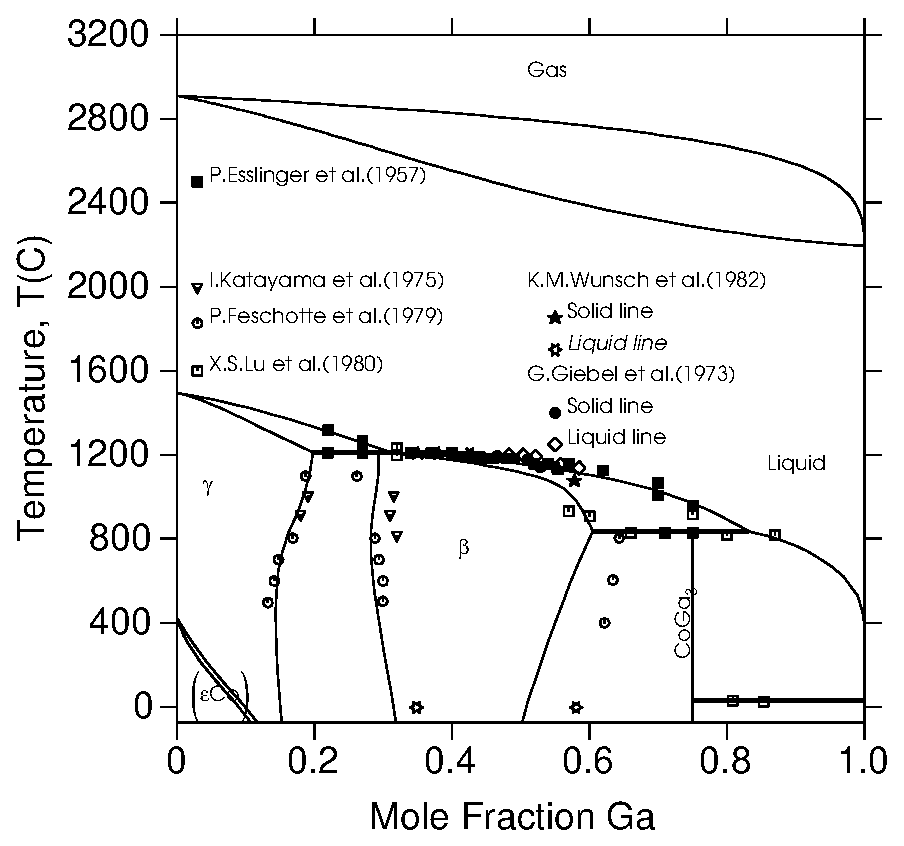
\includegraphics[scale=0.6]{CoGa_binary}
\caption{Calculated CoGa phase diagram compared with experimental data\cite{Cha10}}
\label{Model-cal}
\end{figure}
%%----------------------------------%%
\begin{figure}[b!]
\centering
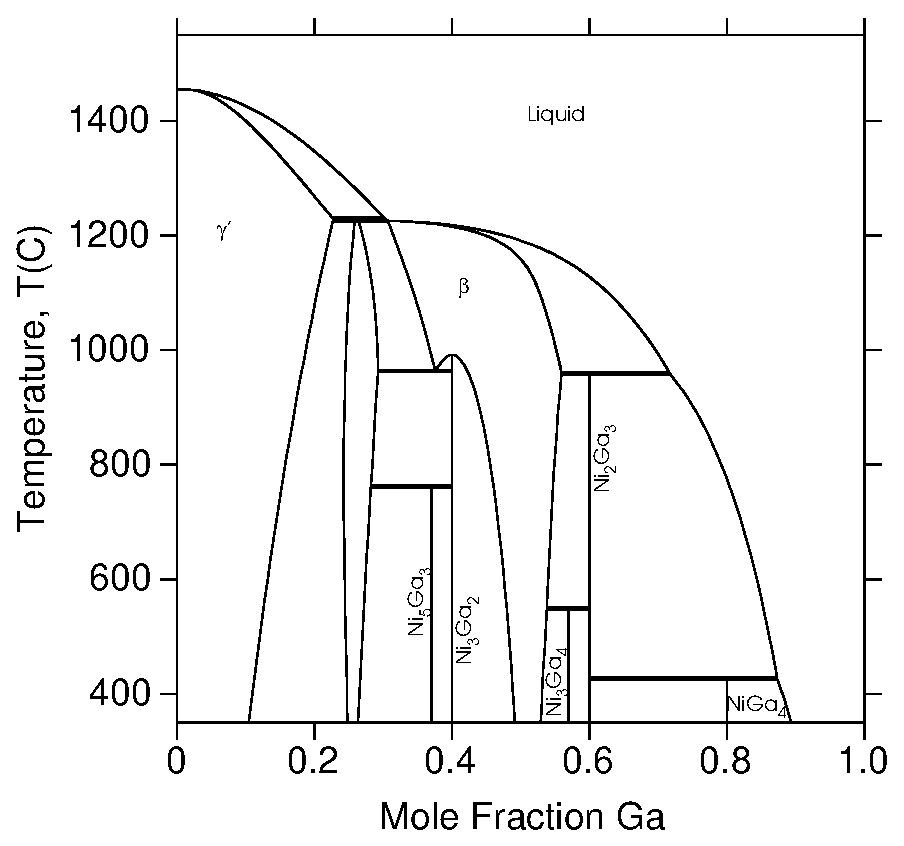
\includegraphics[scale=0.6]{NiGa_binary}
\caption{Binary NiGa phase diagram as calculated by Ipser et al \cite{Ipser04}}
\label{NiGa}
\end{figure}
%%----------------------------------%%
\begin{figure}[t!]
\centering
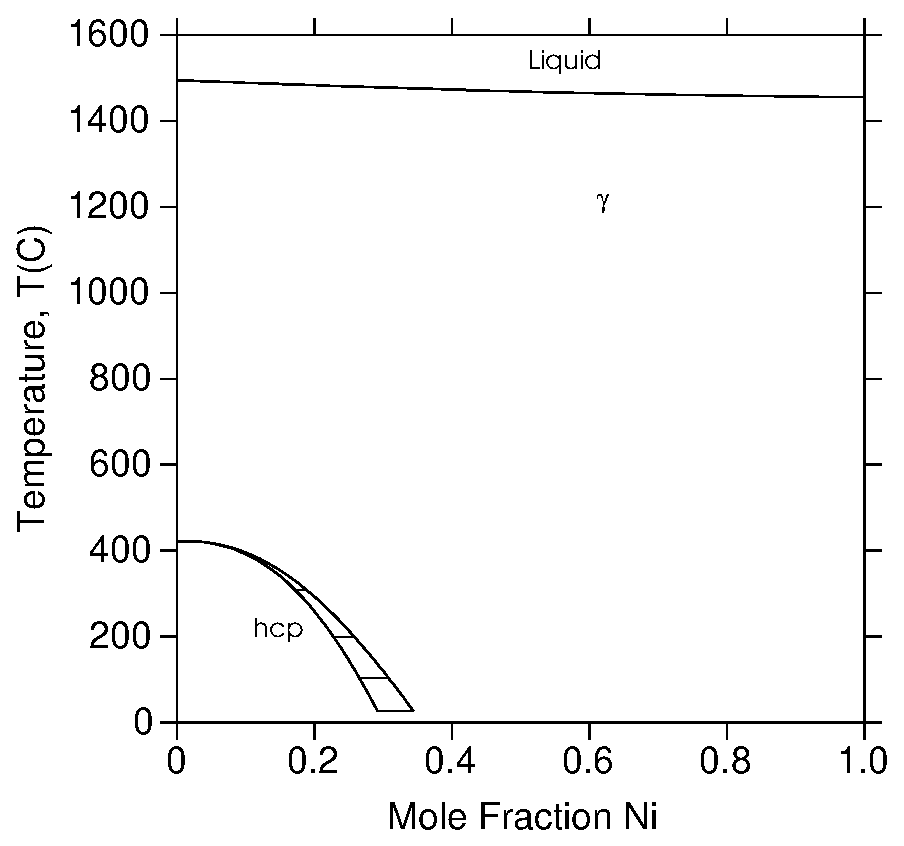
\includegraphics[scale=0.6]{CoNi_binary}
\caption{Binary CoNi phase diagram sourced from the SGTE solution database of ThermoCalc}
\label{CoNi}
\end{figure}
%%----------------------------------%%
Ipser et al. \cite{Ipser04} described the order-disorder transformation between the
non stoichiometric Ni$_{3}$Ga-($\gamma'$)
and fcc($\gamma$) phases, while modeling the NiGa system. The NiGa phase diagram as modeled by Ipser is shown in Fig.\ref{NiGa}. In order to consistently model the ternary,
this phenomenon has not been taken into consideration. The Ni$_5$Ga$_3$ ($\delta$) and Ni$_3$Ga$_2$
($\epsilon$) phases were modeled as stoichiometric phases entering into the ternary. They were
modeled as non-stoichiometric phases as given by the
experimental description of these phases by Ducher et al. \cite{Duch08} at 700$\,^{\circ}\mathrm{C}$
and this could be incorporated in future work. The phase diagram of the CoNibinary 
system as described in the SGTE solution database is shown in Fig.\ref{CoNi}.

%------------------------------------------------------------------------------------------%
\section{Experimental procedure}
\label{Sec:exp_proc}
In order to validate thermodynamic models for the CoNiGa ternary system, different CoNiGa alloy compositions (in at.\%)
were prepared using vacuum arc-melting of 99.9\% purity Co, 99.95\% Ni and 99.999\% purity Ga.
The compositions were chosen from different regions of the ternary system. \textcolor{red}{From our experience on arc-melting of CoNiGa, usually Ga loss is around 3\% of all Ga. Therefore, some extra Ga  was added ($\approx$ 3\% more) to have a composition very close to target composition. WDS analyses confirmed that the measured compositions were very close to nominal compositions. Water cooled Cu crucible was used. No reaction with Ga was expected. Most importantly, Ga was added on top of other elements to minimize any reaction with crucible. In addition, no indication of a reaction on the crucible surface after melting was seen.} These alloys were prepared in the form of
arc melted buttons. The expected phases according to the thermodynamic model and experimentally
observed phases at certain temperatures have been listed in Table \ref{Exp-1}.

The microstructural evolution and chemical analysis were examined using a digital Keyence VH-Z100 optical microscopy (OM)
and a Cameca SX50 scanning electron microscopy (SEM) equipped with four wavelength dispersive X-Ray spectrometers (WDS).
The samples examined using OM were etched in 50\% hydrochloric acid, 33\% ethanol, 8.5\% copper sulfate
and 8.5\% water solution. Crystal structure of different phases were determined using a
Bruker-AXS D8 X-ray diffractometer (XRD)with CuK$_{\alpha}$ (0.15406 nm) radiation.

%------------------------------------------------------------------------------------------%
\section{Optimization procedure}
\label{Modeling}
Experimental data including activities, volume fractions, tie-lines, triple points and
partial molar enthalpies \cite{Oik06,Duch08,Oik01,Liu06,Mik87}
were included in the optimization process, which was performed using the software
ThermoCalc. The software uses a technique of global minimization of Gibbs energy to assess
the thermodynamic model parameters such as the Gibbs energy functions
and interaction parameters. The binary
system parameters were taken from previously developed models of the NiGa and CoGa systems \cite{Ipser04,Cha10}
and these values remained fixed throughout the optimization process.
Initial weights were given to the experimental data based on the accuracy
required for the calculations. The weights were increased as the
optimization process continued, depending on whether the results evaluated were within the
uncertainty limits of the measurements. This was to ensure that self-consistent results
were obtained.

All the model parameters were optimized together, starting with a small number of
optimization iterations and increasing this number as the optimization
progressed. Negative driving force constraints for some phases were enforced
in regions of the ternary to prevent their stability in those regions.

The initial values of the ternary interaction parameters were determined by a trial
and error method, until a reasonable fit was obtained with respect to the experimental
data. The experimental data for vertical sections and volume fractions were given
low weights throughout the optimization process, with higher weights given to
the triple points and tie lines. As the optimization process progressed, the weights for
the triple points were increased as described earlier.

In order for the binary system parameters to impact the ternary, it was necessary to include
ternary interaction parameters as well as the enthalpies of formation for the Gibbs energy
functions of the end members of the
intermetallic phases of the Ni-Ga system. The enthalpies were calculated
using first-principles within the GGA approximation
with projector augmented-wave (PAW) pseudo-potentials, as implemented in the
Vienna ab initio simulation package (VASP) \cite{96Kres,96Kress}. In the case of
GGA, the PW91 corrections have been used \cite{92Perd}. Brillouin zone
integrations were performed using a Monkhorst\textendash{}Pack mesh
\cite{76Monk}. Full relaxations were performed using the
Methfessel\textendash{}Paxton order 1 smearing method \cite{89Meth} and a final
self-consistent static calculation with the tetrahedron smearing method with
Bl\"{o}chl corrections \cite{94Bloc} was performed. The energy cutoff and
k-point mesh used ensured convergence in the total energies calculated within
less than 1 meV. The DFT calculations for the end members were
included in the optimization process. The enthalpies of formation of the relevant phases are listed in Table \ref{table:results Hf}. Experimental values obtained from literature for the same are also listed in the table.
%%----------------------------------%%
\begin{figure}[t!]
\centering
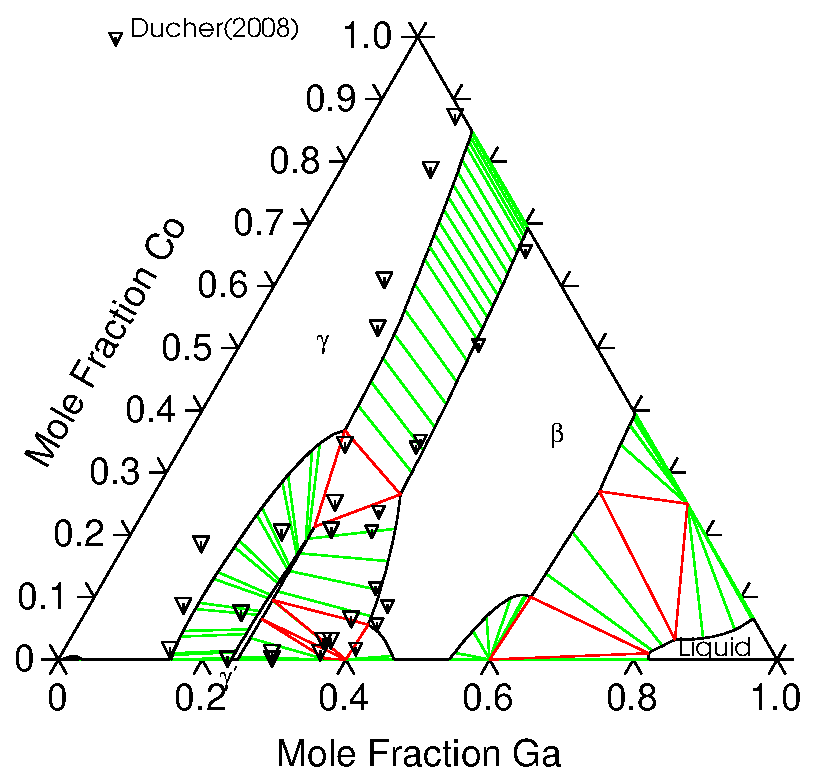
\includegraphics[scale =0.45]{973_isothermal}
\caption{Isothermal section schematic phase diagram of the CoNiGa ternary system at 700$\,^{\circ}\mathrm{C}$}
\label{973}
\end{figure}
%------------------------------------------------------------------------------------------%
\section{Results and discussion}
\subsection{Isothermal sections at 700$\,^{\circ}\mathrm{C}$, 1000$\,^{\circ}\mathrm{C}$ and 1200$\,^{\circ}\mathrm{C}$}
\begin{figure}
\centering
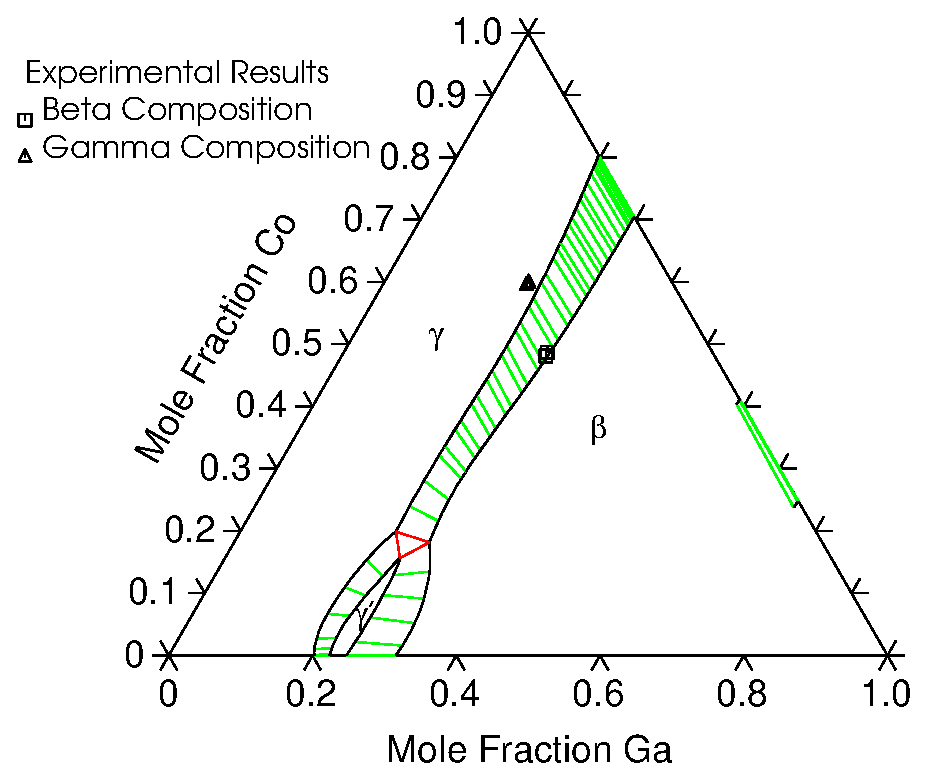
\includegraphics[scale =0.45]{1473_isothermal}
\caption{Isothermal section schematic phase diagram of the CoNiGa ternary system at 1000$\,^{\circ}\mathrm{C}$}
\label{1273}
\end{figure}
%%----------------------------------%%
\begin{figure}
\centering
\includegraphics[scale =0.45]{1273_isothermal}
\caption{Isothermal section schematic phase diagram of the CoNiGa
ternary system at 1200$\,^{\circ}\mathrm{C}$}
\label{1473}
\end{figure}
%%----------------------------------%%
\subsubsection{Microstructure and two-phase equilibrium}
The ternary phase diagram was optimized for a wide range of temperatures and the isothermal sections
are shown in Figs. \ref{973},\ref{1273},\ref{1473} as compared with experimental data.
Equilibrium concentrations of the $\gamma$, $\beta$ and $\gamma'$ phases at
700$\,^{\circ}\mathrm{C}$, 1000$\,^{\circ}\mathrm{C}$ and 1200$\,^{\circ}\mathrm{C}$
have been listed in Table \ref{Exp-2}. The optimized binary and ternary interaction parameters,
including the Gibbs energy functions have been calculated using the model and are listed in Table \ref{Opt:Par}.
It can be observed from the three isothermal sections of the ternary that there are
two distinct phases present: $\gamma$ and $\beta$. This two-phase region extends into
the ternary over a wide range of composition, from the CoGa side towards the Ni-rich side.
The $\gamma$ phase is present in the Co and Ni rich regions and the $\beta$ phase is present
in the central region of the ternary. The $\gamma'$ phase can be observed at compositions
up to 30 at. \% Ni. Additional phases $\delta$ and $\epsilon$ are also observed at
700$\,^{\circ}\mathrm{C}$ (Fig. \ref{973}). These intermetallic phases are observed
below 700$\,^{\circ}\mathrm{C}$ between 30-40 at.\% Ga as also reported by
Ducher et.al\cite{Duch08}. The single phase regions are parallel to the CoNi region,
with no solubility change in Ga. The $\beta$+$\gamma$ two-phase region agrees well
with the results reported by Ducher \cite{Duch08}. At 1000$\,^{\circ}\mathrm{C}$
(Fig \ref{1273}), the concentrations at the two-phase $\beta$+$\gamma$ phase boundaries
compare well with the experimental results by Oikawa et. al \cite{Oik06,Oik01}.
The equilibrium data obtained between the $\beta$,$\gamma$ and $\gamma'$ phases
(three-phase triple point region) is in agreement with the results by Ducher
\cite{Duch08}. At 1200$\,^{\circ}\mathrm{C}$ , it can be seen that the $\beta$
and $\gamma$ phase compositions compare well with our experimental work (Fig \ref{1473}).
It is observed that the two-phase $\beta$+$\gamma$ region widens with decreasing
temperature as also reported by Oikawa \cite{Oik06,Oik01}.

\subsubsection{Experimental results}
Fig.\ref{Opt-Mic} displays an optical micrograph of the Co$_{0.30}$Ni$_{0.45}$Ga$_{0.25}$
sample after homogenization at 1077$\,^{\circ}\mathrm{C}$ for 24 hrs
followed by water quenching indicating two phase microstructure ($\beta$+$\gamma$).
Figures \ref{xrd_Co30}-\ref{xrd_Co5} show X-ray diffraction pattern of Co$_{0.20}$Ni$_{0.65}$Ga$_{0.15}$,
Co$_{0.30}$Ni$_{0.45}$Ga$_{0.25}$, Co$_{0.80}$Ni$_{0.15}$Ga$_{0.05}$ and
Co$_{0.05}$Ni$_{0.62}$Ga$_{0.33}$ alloys, respectively.
%%----------------------------------%%
\begin{figure}[!htbp]
\centering
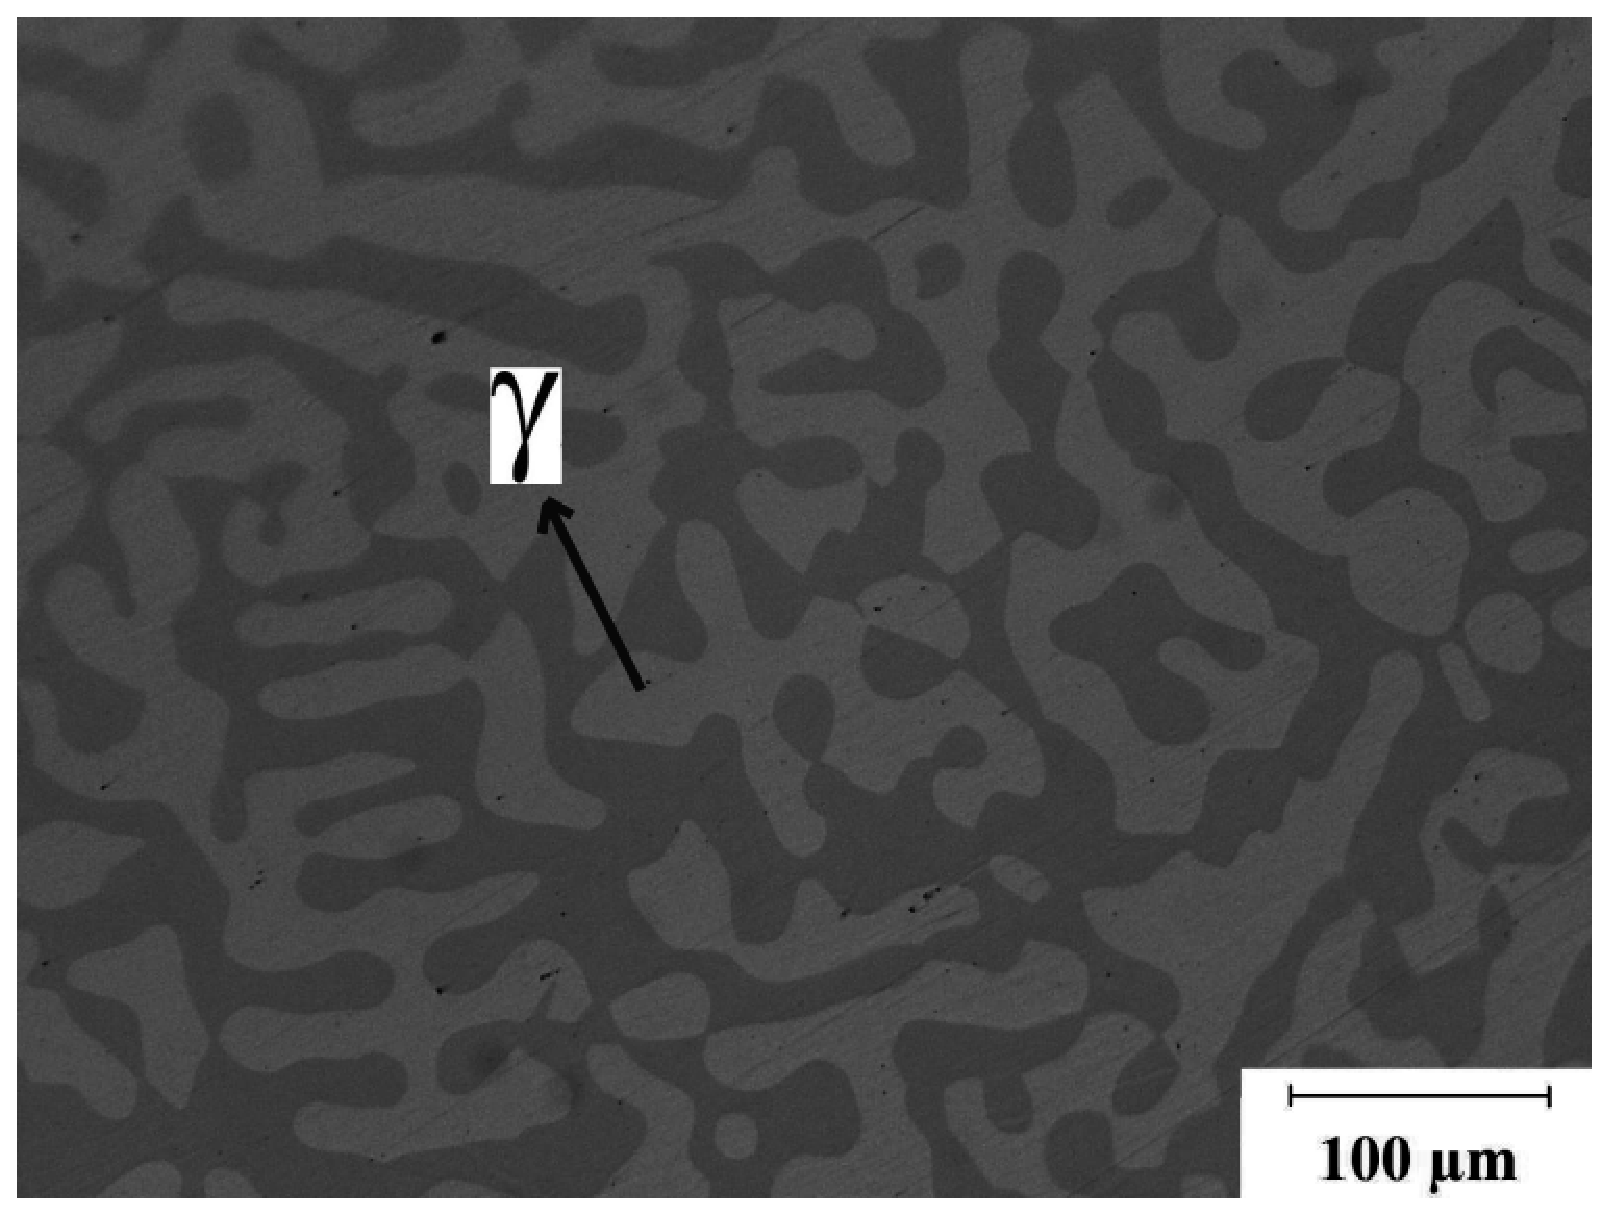
\includegraphics[scale=0.35]{CoNiGa_micrograph}
\caption{Optical micrograph of Co$_{0.30}$Ni$_{0.45}$Ga$_{0.25}$ sample after homogenization
at 1077$\,^{\circ}\mathrm{C}$ for 24 hrs followed by water quenching indicating
two phase microstructure ($\beta$+$\gamma$)}
\label{Opt-Mic}
\end{figure}
%%----------------------------------%%
\begin{figure}[!htbp]
\centering
     \subfigure[(a)]{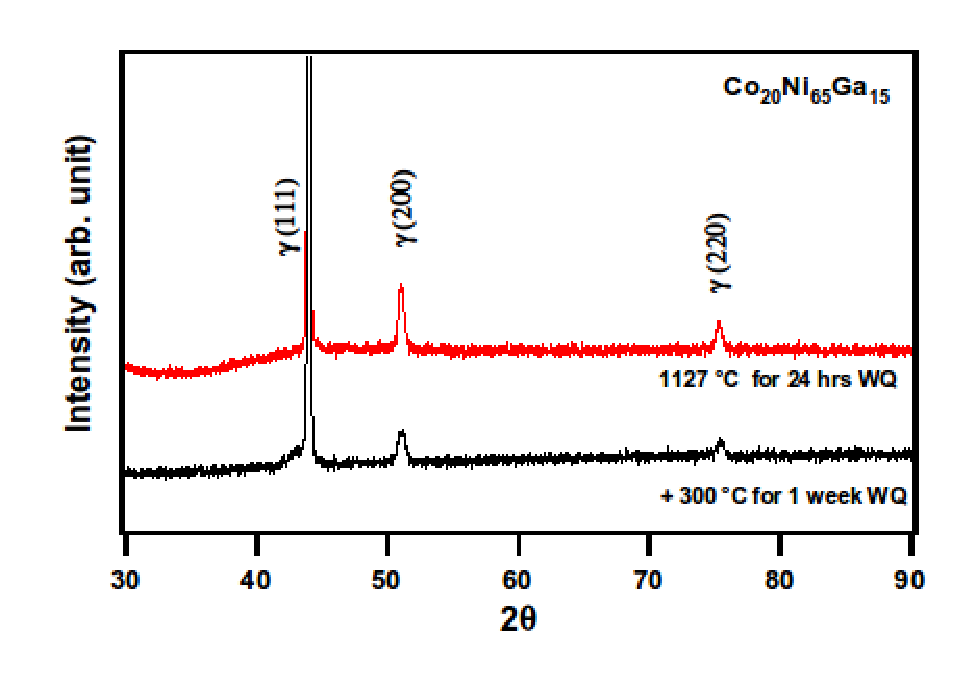
\includegraphics[width=0.45\textwidth]{xrd_Co20}\label{xrd_Co20}}
     \subfigure[(b)]{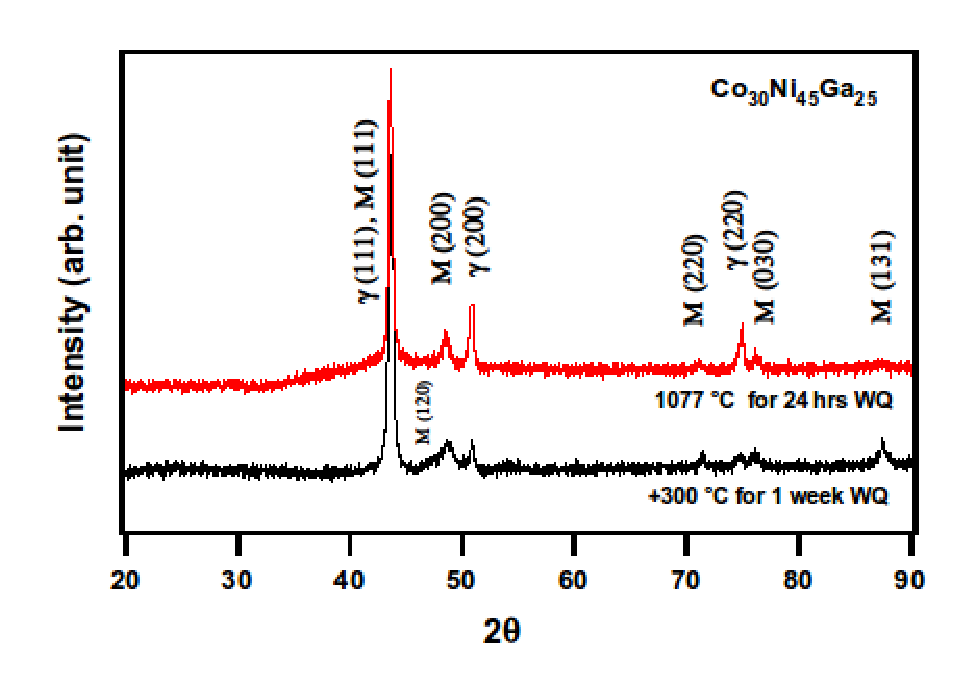
\includegraphics[width=0.45\textwidth]{xrd_Co30}\label{xrd_Co30}}
\caption{X-ray diffraction pattern of the (a) Co$_{0.2}$Ni$_{0.65}$Ga$_{0.15}$ and (b) Co$_{0.3}$Ni$_{0.45}$Ga$_{0.25}$ samples indicating the structures of the constitutive phases after different heat treatments. M: L10 Martensite, $\gamma$: A1 structure (disordered fcc)}
\end{figure}
%%----------------------------------%%
\begin{figure}[!htbp]
\centering
     \subfigure[(a)]{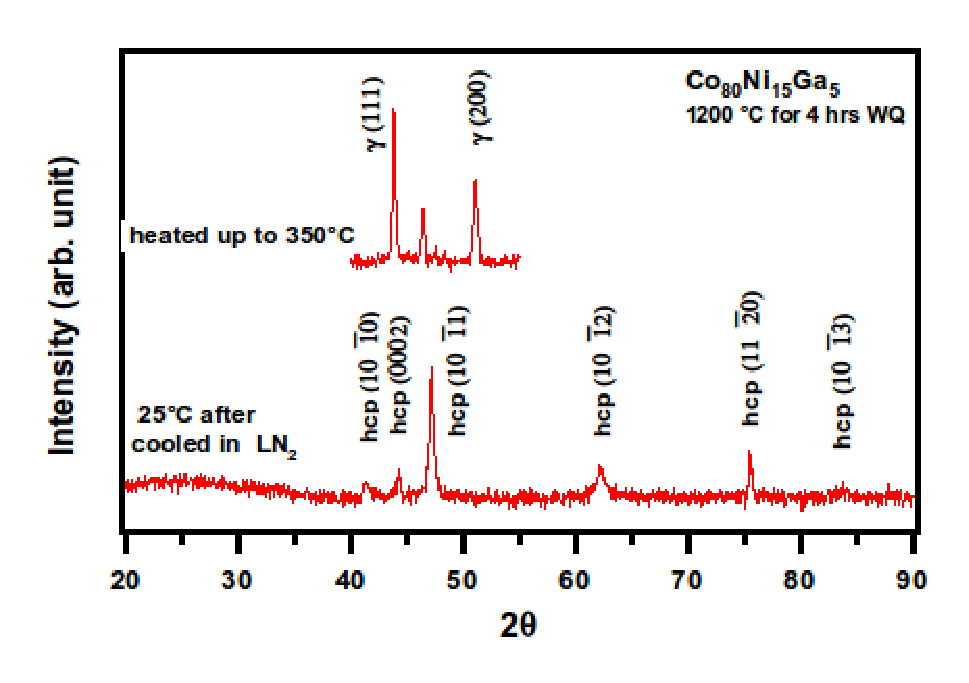
\includegraphics[width=0.45\textwidth]{xrd_Co80}\label{xrd_Co80}}
     \subfigure[(b)]{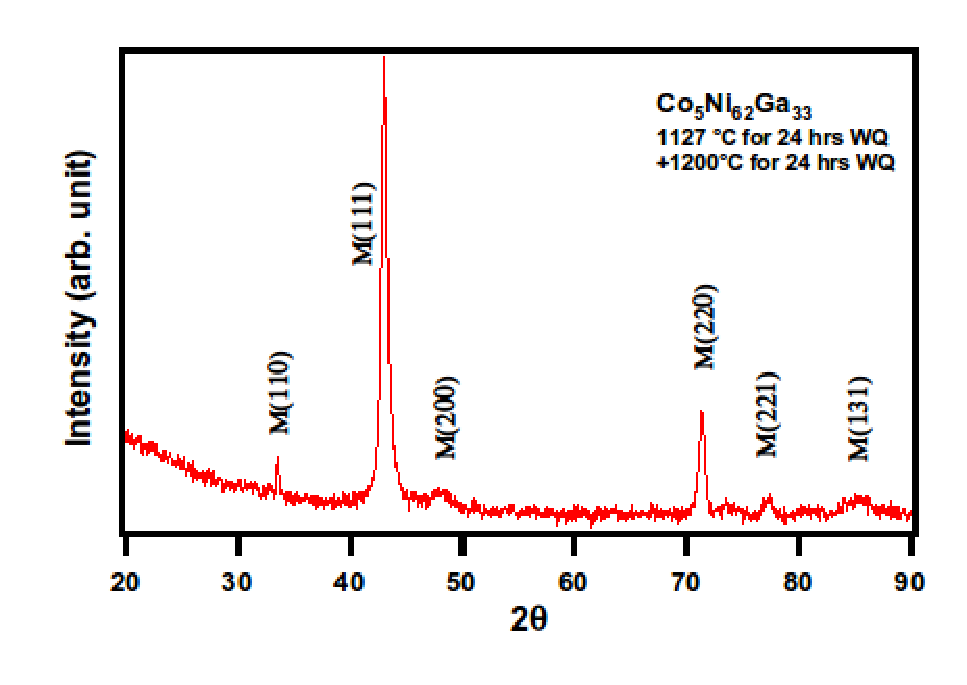
\includegraphics[width=0.45\textwidth]{xrd_Co5}\label{xrd_Co5}}
\caption{X-ray diffraction pattern of the (a) Co$_{0.8}$Ni$_{0.15}$Ga$_{0.05}$  and (b) Co$_{0.05}$Ni$_{0.62}$Ga$_{0.33}$ samples indicating the structures of the constitutive phases after different heat treatments. M: L10 Martensite, hcp: A3 structure}
\end{figure}
%%----------------------------------%%
Overall, there is a good agreement between expected and observed phases at the temperatures considered (Table \ref{Exp-1}).
According to the thermodynamics model the stable phase at 1200$\,^{\circ}\mathrm{C}$ for Co$_{0.05}$Ni$_{0.62}$Ga$_{0.33}$
and at 1127$\,^{\circ}\mathrm{C}$ for Co$_{0.20}$Ni$_{0.65}$Ga$_{0.15}$ are $\beta$ and $\gamma$ phase respectively,
which agree well with experimental results. For Co$_{0.20}$Ni$_{0.65}$Ga$_{0.15}$, the thermodynamic
model indicates two phase microstructure $\gamma$ and ($\gamma'$) phases at 300$\,^{\circ}\mathrm{C}$ .
Ageing at 300$\,^{\circ}\mathrm{C}$ for 1 week does not change the microstructure and stable structure
is only  the $\gamma$ phase. For Co$_{0.30}$Ni$_{0.45}$Ga$_{0.25}$, the X-Ray diffraction pattern (Fig.\ref{xrd_Co30}) reveals
two phase microstructure of $\beta$ and $\gamma$ phases, which has a good agreement with the thermodynamics model
for 1077$\,^{\circ}\mathrm{C}$. However, aging at 300$\,^{\circ}\mathrm{C}$ for one week does not change the microstructure
and the constitutive phases Fig.\ref{xrd_Co30}. There is an inconsistency with the thermodynamics model which indicates
Ni$_{5}$Ga$_{3}$ formation from $\beta$ structure and $\gamma$ phase when the sample is aged at 300$\,^{\circ}\mathrm{C}$.
The discrepancy between the model and the experiment for 300$\,^{\circ}\mathrm{C}$ could be attributed to the possibility that an aging time of 
 one week is not sufficient to form such precipitates. Otherwise the thermodynamics model should be
revised for this temperature. The expected phase at 1200$\,^{\circ}\mathrm{C}$
for Co$_{0.80}$Ni$_{0.15}$Ga$_{0.05}$ alloy is single $\gamma$ phase structure
however hcp phase has been observed experimentally as shown in Fig.\ref{xrd_Co80}. This is due to martensitic transformation of $\gamma$ phase to hcp phase. Fig. 9a shows XRD pattern of  $Co_{0.80}Ni_{0.15}Ga_{0.05}$ after heating up to 350$\,^{\circ}\mathrm{C}$, which indicated that hcp structure transforms back to fcc $\gamma$ structure upon heating up to 350$\,^{\circ}\mathrm{C}$. 

\subsection{Vertical sections, activities, partial enthalpy, phase fractions
and sublattice site fraction of vacancy plots for different alloy compositions}
Fig \ref{vert_20Ni} shows a vertical section at 20 at. \% Ni. Studies
\cite{Duch08,Oik01} have shown that this section is the most important
section for microstructure control in the CoNiGa ternary. The calculated
phase boundaries have been compared with previously developed work. From Fig \ref{vert_20Ni} 
it can be seen that the solubility of Ga in the $\beta$ phase decreases with a decrease in temperature.

The chemical activity of Ga (Ref.State:Liquid) in the ternary $\beta$ phase was determined
for varying compositions of Ga at 900 $\,^{\circ}\mathrm{C}$ and can be seen in
Figs. \ref{acr_co75}, \ref{acr_co25} and \ref{acr_co50}. It can be observed that the values of
activities agree well with the results by Mikula et al.\cite{Mik87} for 45, 50 and 55 at.\% Ga.
Deviations are seen at 40 and 60 at.\% Ga. The partial enthalpy of the ternary $\beta$ phase was
determined for varying compositions of Ga  at 900$\,^{\circ}\mathrm{C}$ and can be
seen in Figs. \ref{hmr_co75},\ref{hmr_co25} and \ref{hmr_co50}. It can be observed that the partial
enthalpies are closer to Mikula's results \cite{Mik87} for 40, 45 and 50 at.\% Ga,
than at 55 and 60 at.\% Ga. Mikula et al. \cite{Mik87} through their emf studies
of the $\beta$ phase, noticed considerable deviations of partial enthalpy and activity
of Ga at 55 and 60 at. \% when compared to theoretical
calculations. A conclusion was hence made that that the phase boundary of the
$\beta$ phase in the ternary, could be close to or below 55 at. \% Ga.
In the present work, the $\beta$ phase boundaries were found between 38 and
55 at. \% Ga, hence agreeing with the experimental work by Mikula.

In order to understand the triple defect structure of the ternary $\beta$ phase,
the sublattice site fraction of vacancies in the second sublattice of the $\beta$ phase with varying composition and temperature was calculated and is as shown in Figs. \ref{sf-comp_CoNiGa} and \ref{sf-temp_CoNiGa} respectively.
Also, the phase fractions of all the phases at the compositions Co$_{5}$Ga$_{33}$Ni$_{62}$,
Co$_{20}$Ga$_{15}$Ni$_{65}$, Co$_{30}$Ga$_{25}$Ni$_{45}$,
Co$_{80}$Ga$_{5}$Ni$_{15}$ and 1200$\,^{\circ}\mathrm{C}$ have been calculated
(based on the experimental compositions from Dr. Karaman's group)
as shown in Figs. \ref{NP_Co5}, \ref{NP_Co20}, \ref{NP_Co30} and \ref{NP_Co80} respectively.
%%----------------------------------%%
\begin{figure}
\centering
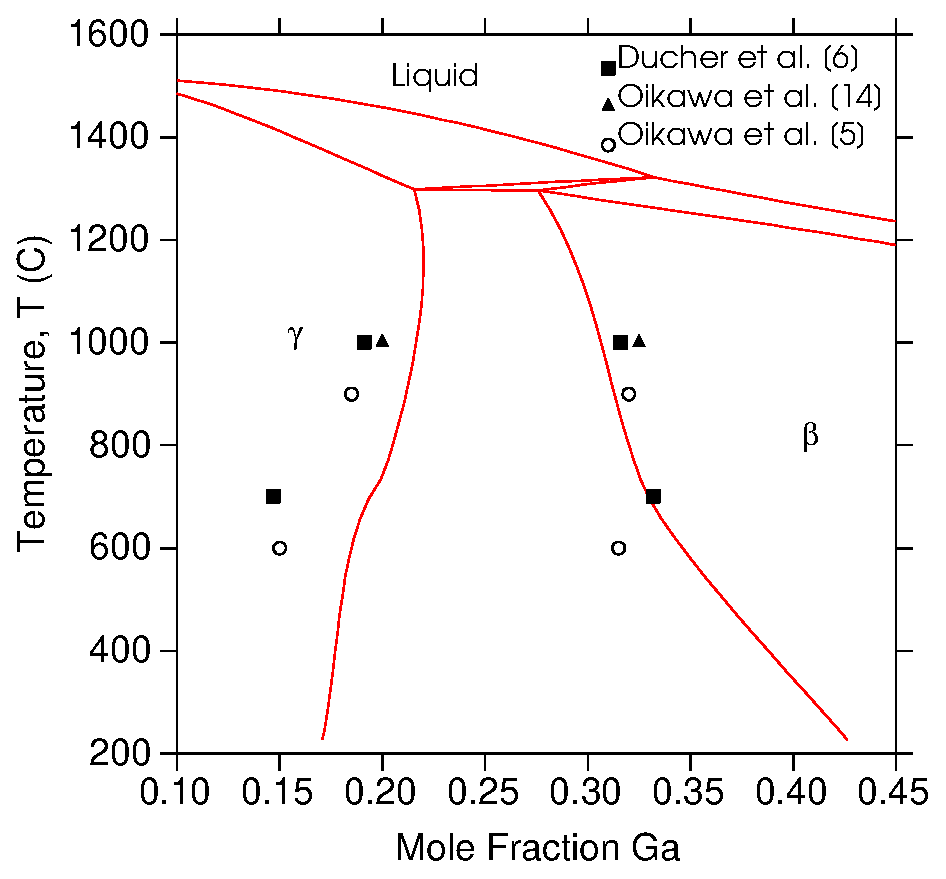
\includegraphics[scale=0.45]{CoNiGa_vertical_section}
\caption{Vertical section of the CoNiGa system at 20 at. \% Ni}
\label{vert_20Ni}
\end{figure}
%----------------------------------%%
\begin{figure}
\centering
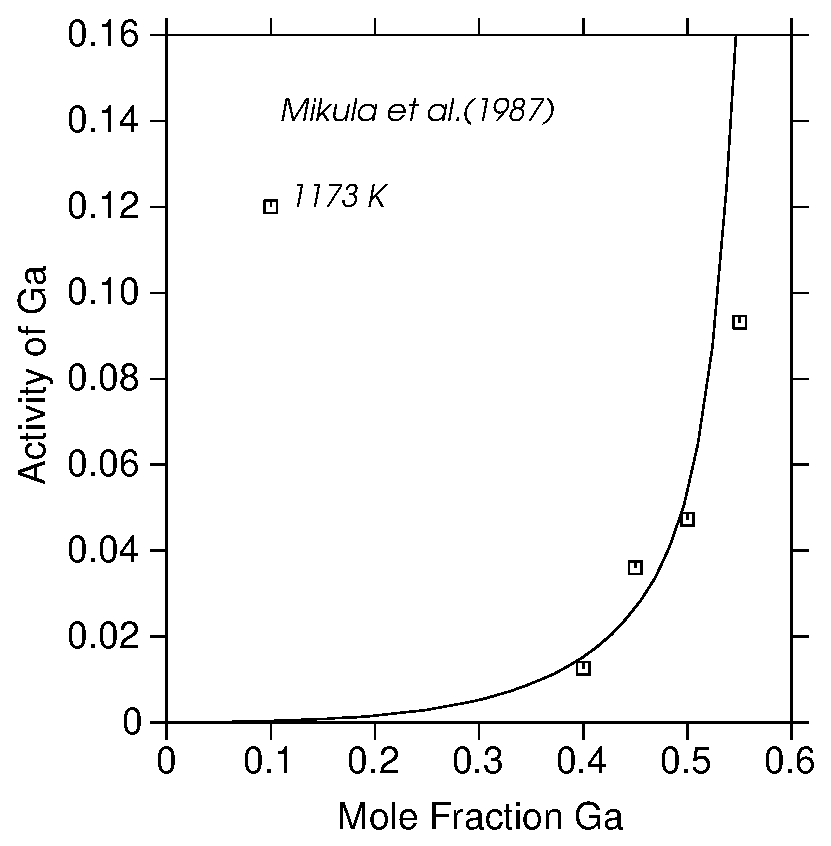
\includegraphics[scale=0.45]{acr_beta_Co75}
\caption{Activity of Ga in the $\beta$ phase at x$_{Co}$/x$_{Ni}$=3:1 and 900$\,^{\circ}\mathrm{C}$}
\label{acr_co75}
\end{figure}
%%----------------------------------%%
\begin{figure}
\centering
\includegraphics[scale=0.45]{acr_beta_Co25}
\caption{Activity of Ga in the $\beta$ phase at x$_{Co}$/x$_{Ni}$=1:3 and 900$\,^{\circ}\mathrm{C}$}
\label{acr_co25}
\end{figure}
%----------------------------------%%
\begin{figure}
\centering
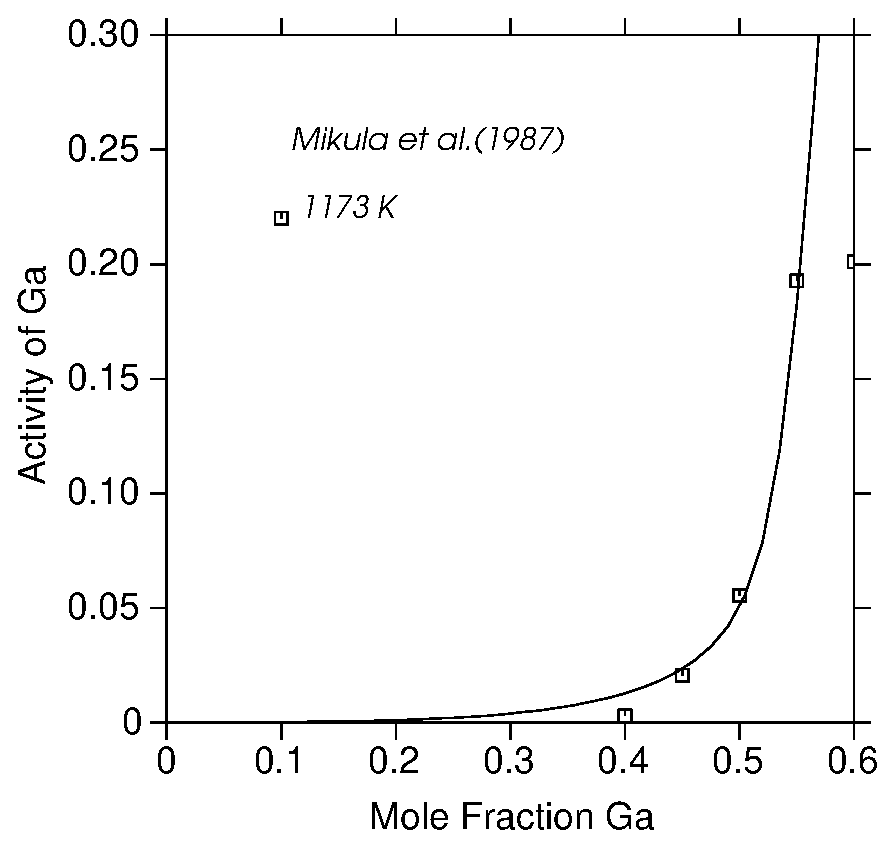
\includegraphics[scale=0.45]{acr_beta_Co50}
\caption{Activity of Ga in the $\beta$ phase at x$_{Co}$/x$_{Ni}$=1:1 and 900$\,^{\circ}\mathrm{C}$}
\label{acr_co50}
\end{figure}
%%----------------------------------%%
\begin{figure}
\centering
\includegraphics[scale=0.45]{hmr_beta_Co75}
\caption{Partial Enthalpy of $\beta$ phase at x$_{Co}$/x$_{Ni}$=3:1 and 900$\,^{\circ}\mathrm{C}$}
\label{hmr_co75}
\end{figure}
%----------------------------------%%
\begin{figure}
\centering
\includegraphics[scale=0.45]{hmr_beta_Co25}
\caption{Partial Enthalpy of $\beta$ phase at x$_{Co}$/x$_{Ni}$=1:3 and 900$\,^{\circ}\mathrm{C}$}
\label{hmr_co25}
\end{figure}
%%----------------------------------%%
\begin{figure}
\centering
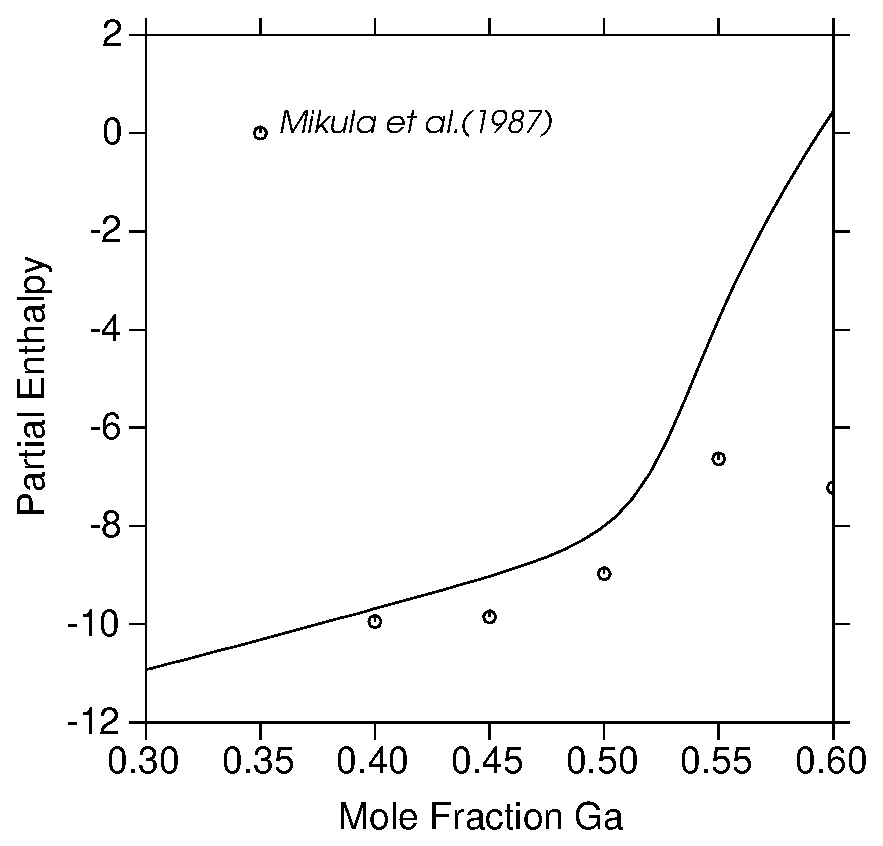
\includegraphics[scale=0.45]{hmr_beta_Co50}
\caption{Partial Enthalpy of $\beta$ phase at x$_{Co}$/x$_{Ni}$=1:1 and 900$\,^{\circ}\mathrm{C}$}
\label{hmr_co50}
\end{figure}
%----------------------------------%%
\begin{figure}
\centering
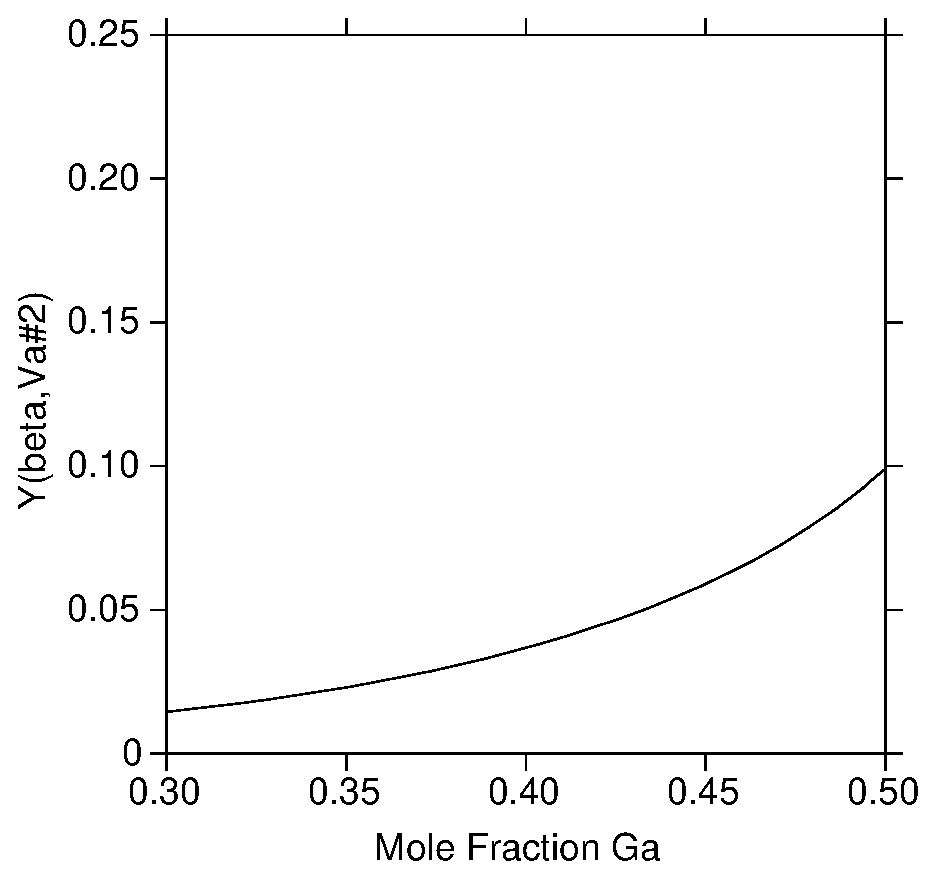
\includegraphics[scale=0.45]{sf_comp_CoNiGa}
\caption{Sublattice site fraction of vacancies in the second sublattice of the
ternary $\beta$ phase as a function of composition at 900$\,^{\circ}\mathrm{C}$}
\label{sf-comp_CoNiGa}
\end{figure}
%----------------------------------%%
\begin{figure}
\centering
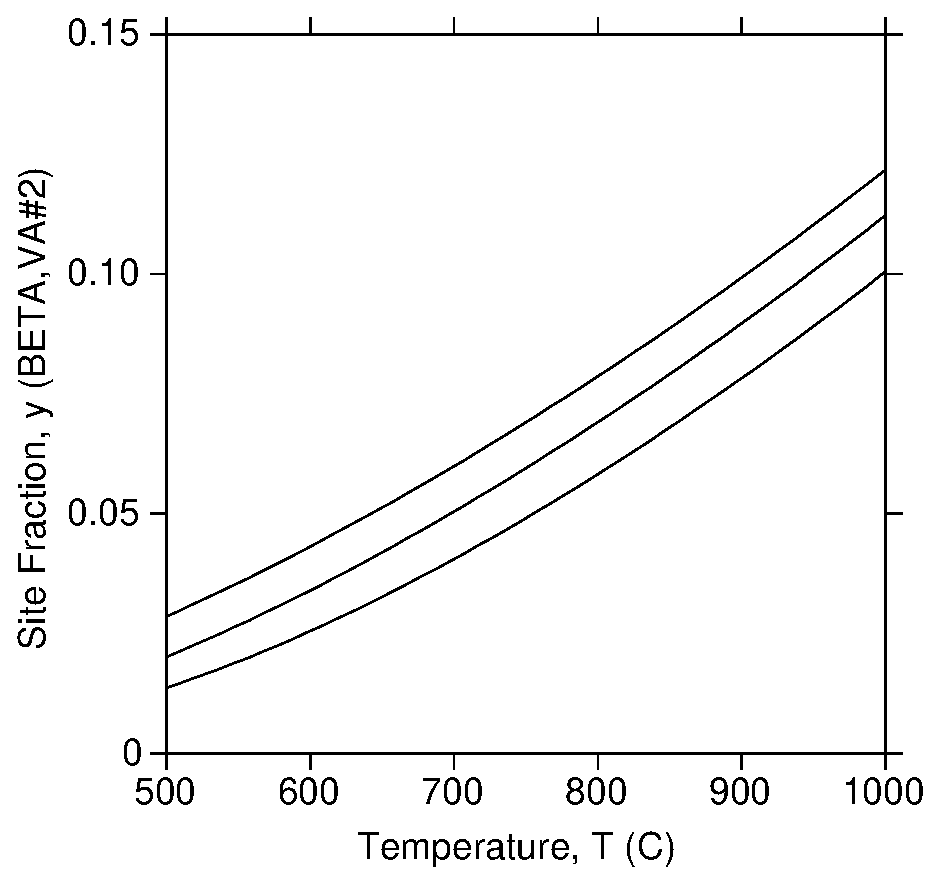
\includegraphics[scale=0.45]{sf_temp_CoNiGa}
\caption{Sublattice site fraction of vacancies in the second sublattice of the
ternary $\beta$ phase as a function of temperature  at 50, 52, 54 at. \% Co and 50 at. \% Ga} 
\label{sf-temp_CoNiGa}
\end{figure}
%----------------------------------%%
\begin{figure}
\centering
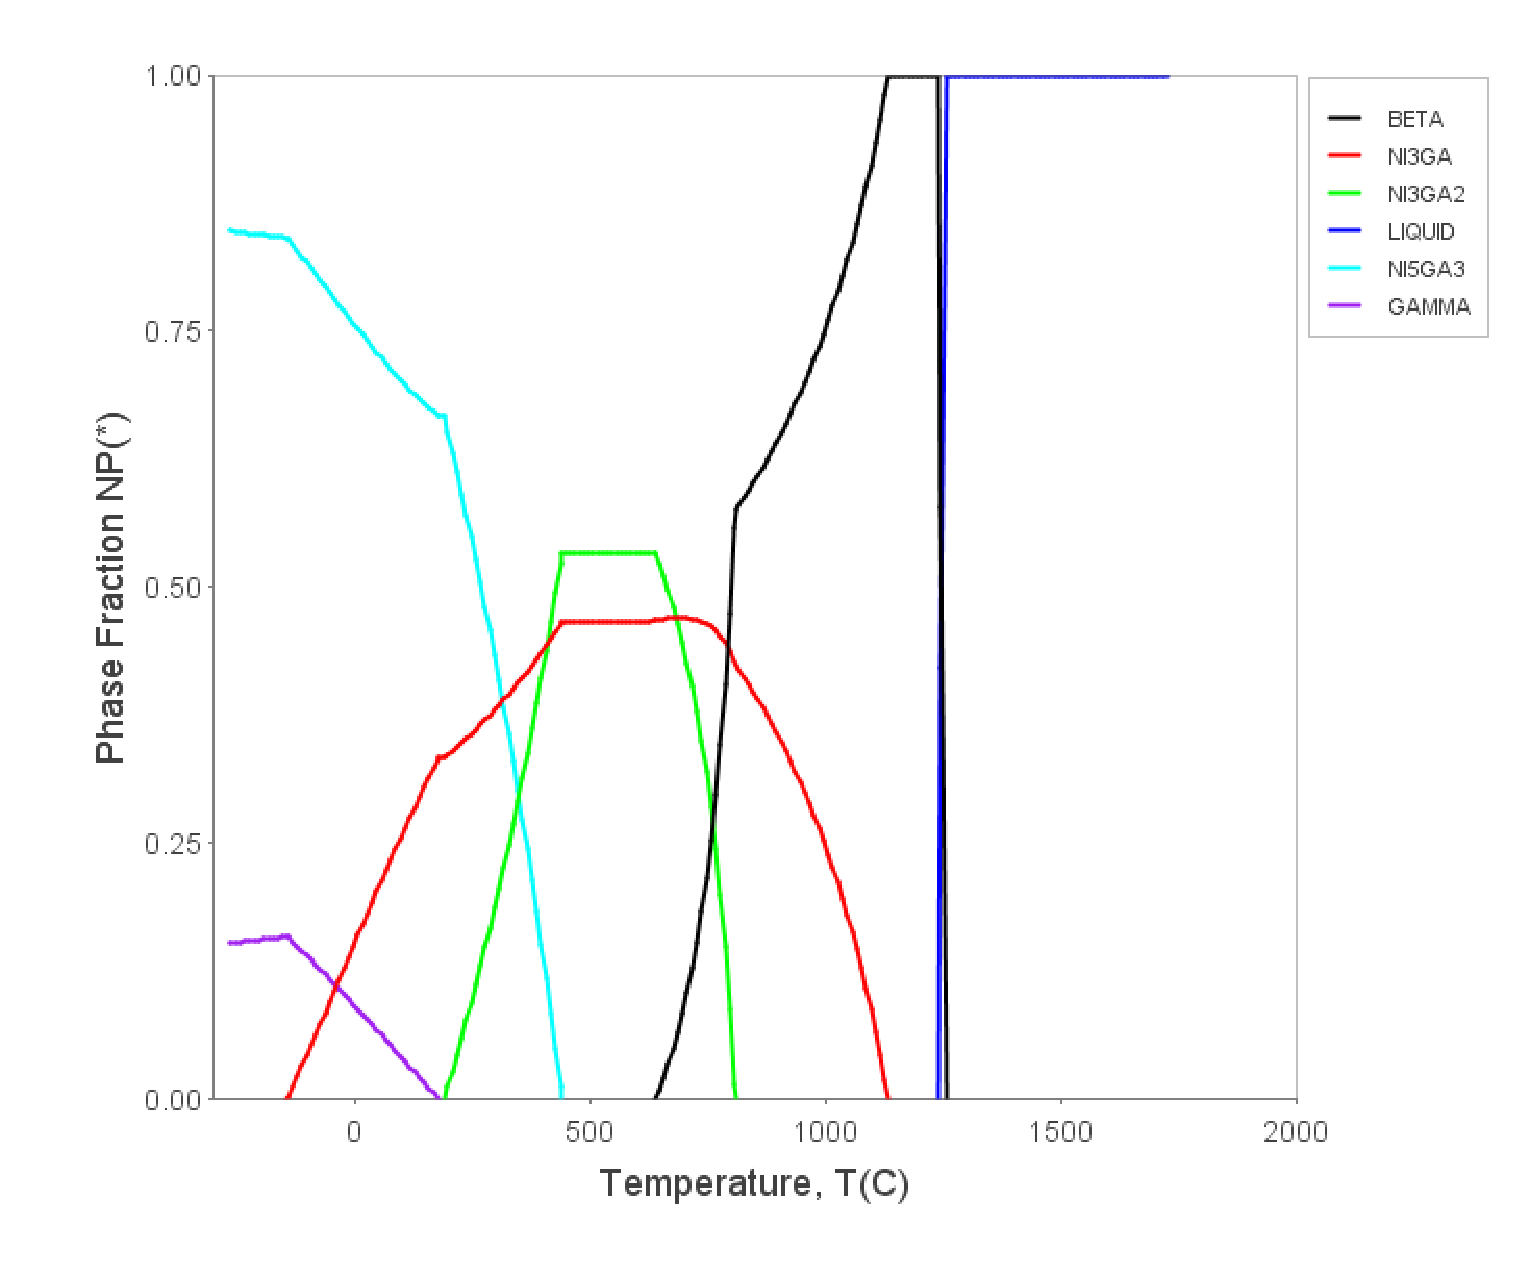
\includegraphics[scale=0.4]{Co_5}
\caption{Phase fractions of all the phases in the ternary at Co$_{0.05}$Ga$_{0.33}$Ni$_{0.62}$ and 1200$\,^{\circ}\mathrm{C}$}
\label{NP_Co5}
\end{figure}
%----------------------------------%%
\begin{figure}
\centering
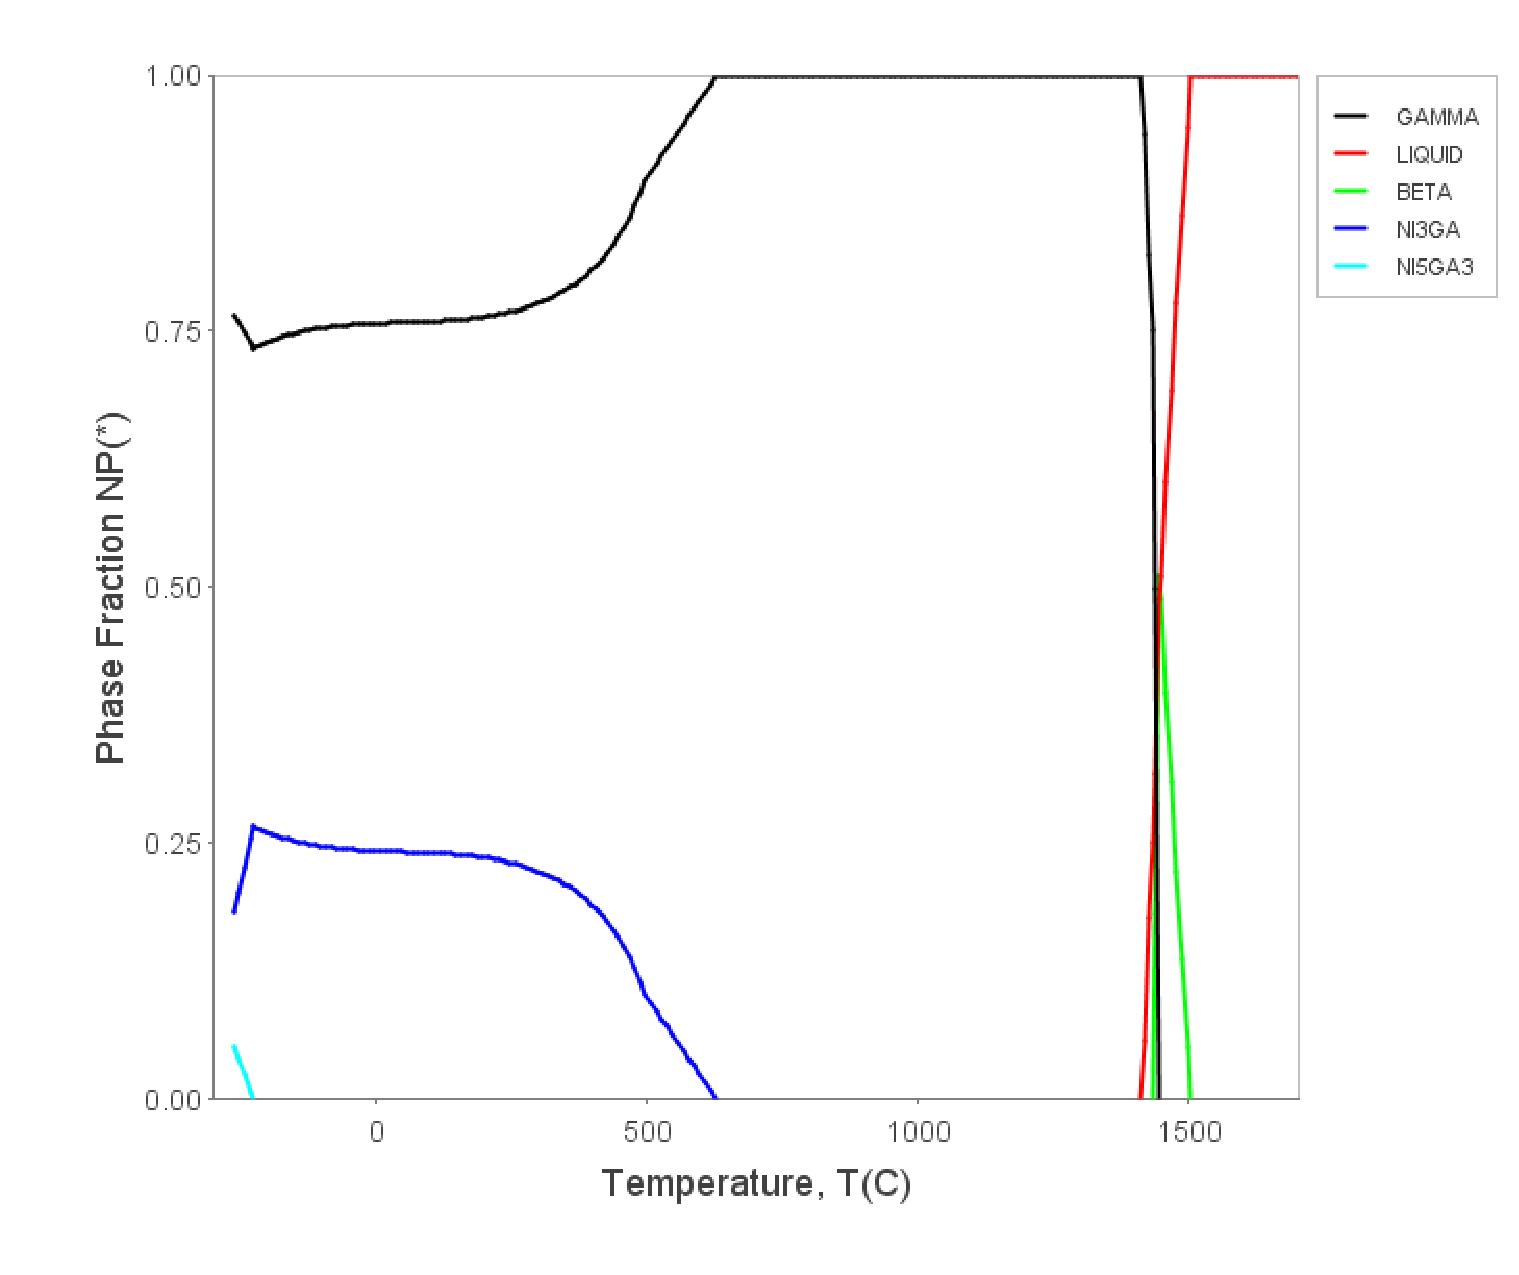
\includegraphics[scale=0.4]{np_ternary_Co20}
\caption{Phase fractions of all the phases in the ternary at Co$_{20}$Ga$_{15}$Ni$_{65}$ and 1200$\,^{\circ}\mathrm{C}$}
\label{NP_Co20}
\end{figure}
%%----------------------------------%%
\begin{figure}
\centering
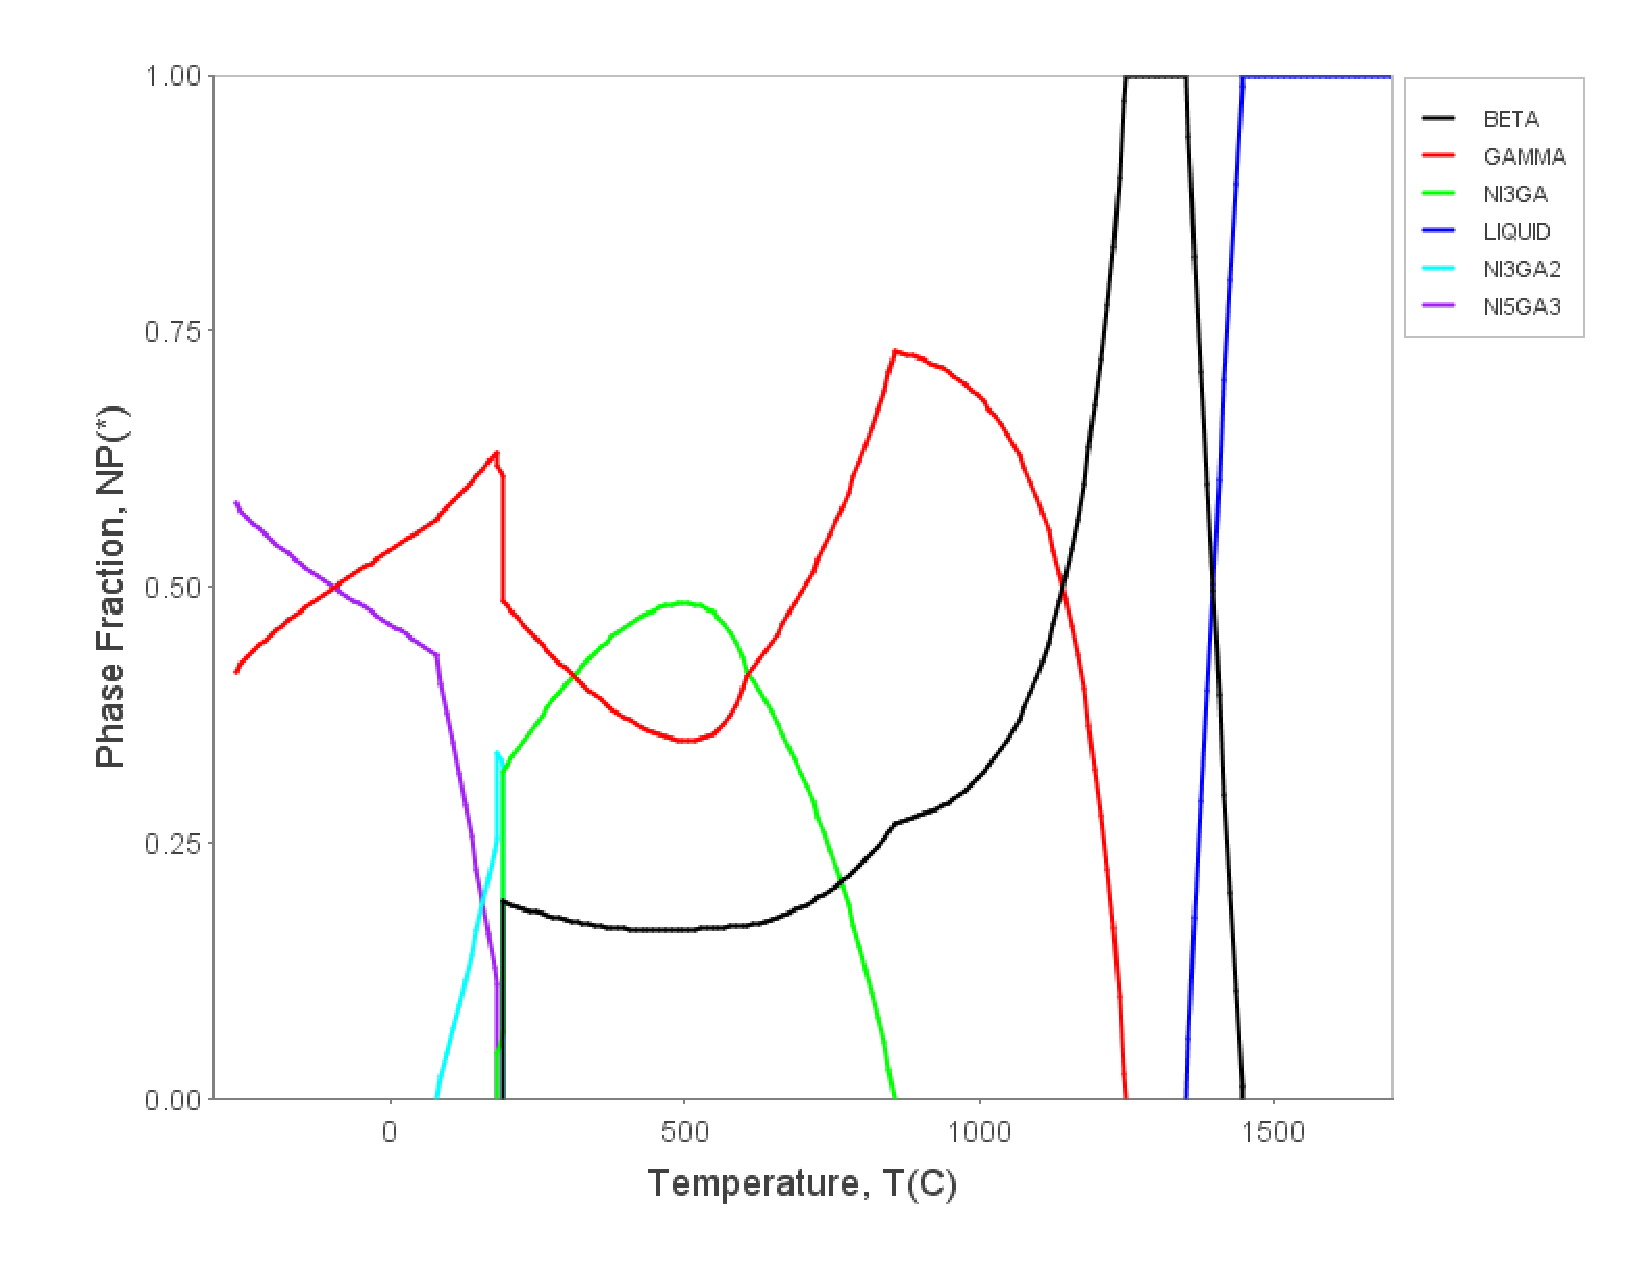
\includegraphics[scale=0.4]{np_ternary_Co30}
\caption{Phase fractions of all the phases in the ternary at Co$_{30}$Ga$_{25}$Ni$_{45}$ and 1200$\,^{\circ}\mathrm{C}$}
\label{NP_Co30}
\end{figure}
%%----------------------------------%%
\begin{figure}
\centering
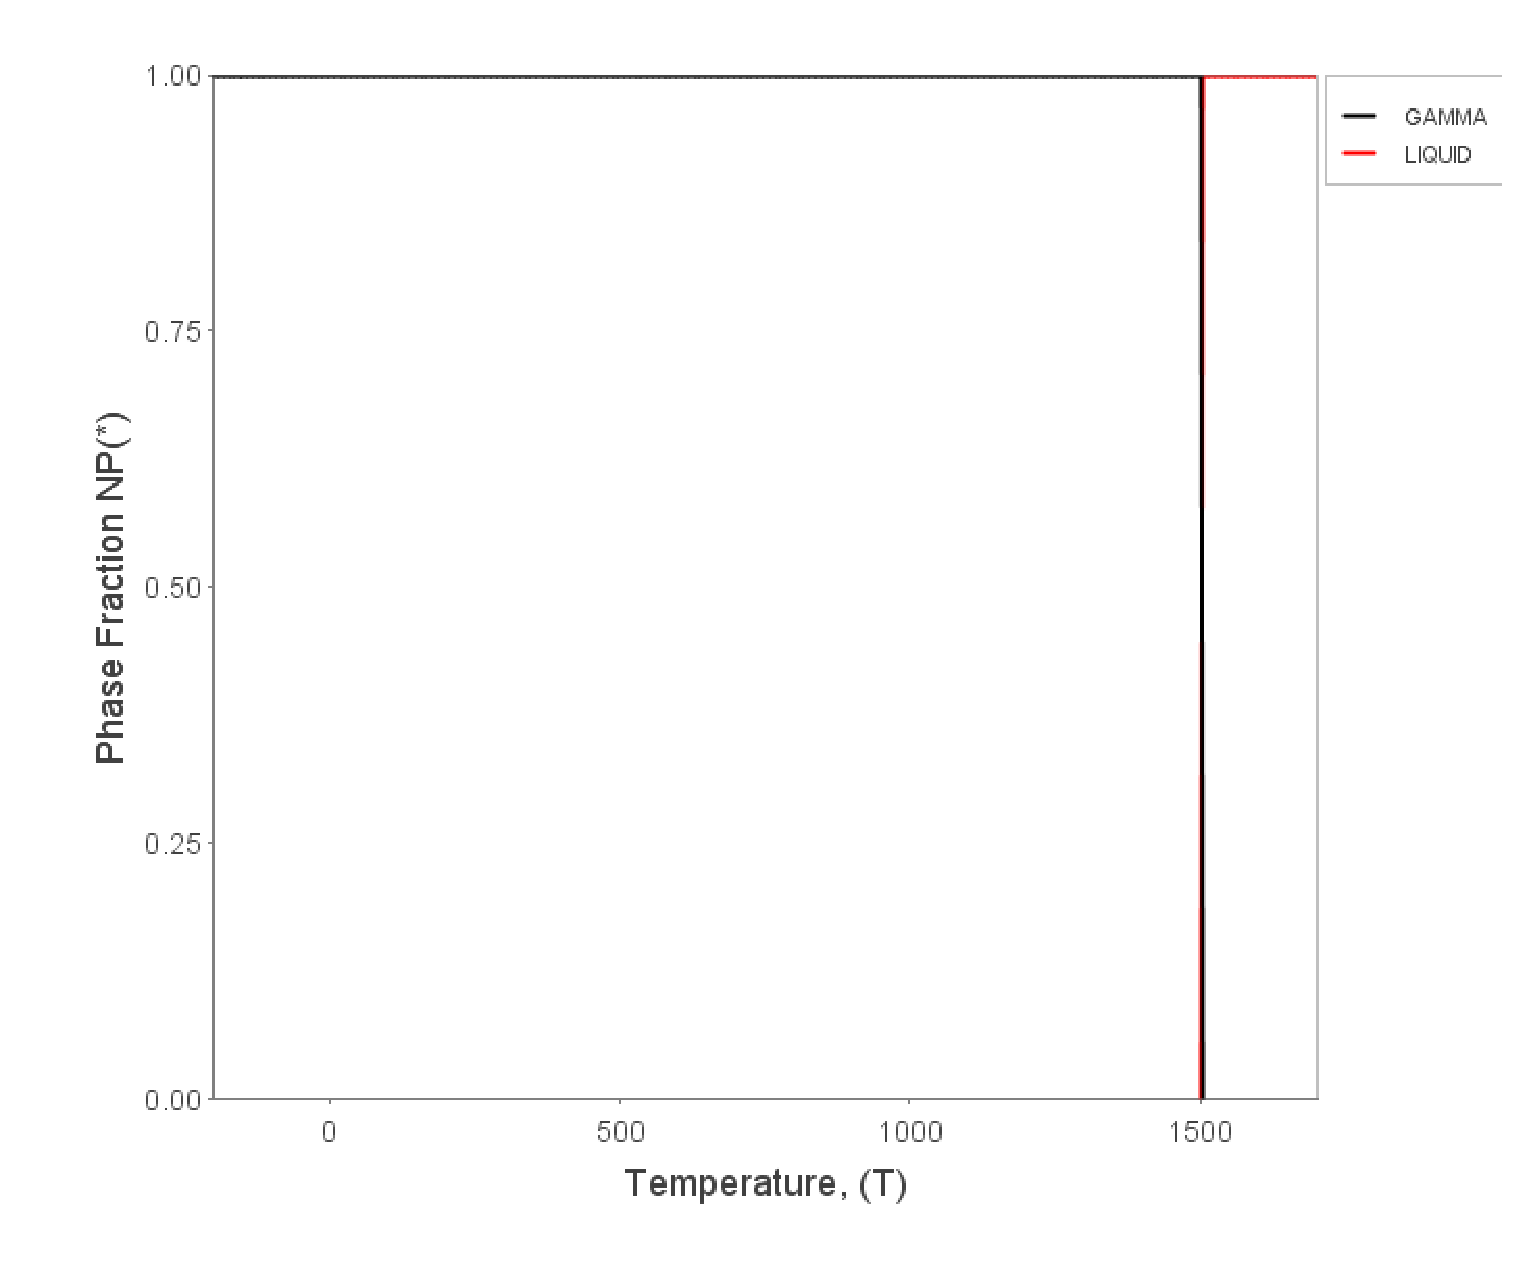
\includegraphics[scale=0.35]{np_ternary_Co80}
\caption{Phase fractions of all the phases in the ternary at Co$_{80}$Ga$_{5}$Ni$_{15}$ and 1200$\,^{\circ}\mathrm{C}$}
\label{NP_Co80}
\end{figure}
%------------------------------------------------------------------------------------------%
\section{Conclusion}
\label{Sec:conclusion}
The phase equilibria among the $\gamma$ (fcc), $\beta$, $\gamma'$ (Ni$_3$Ga),
$\delta$ (Ni$_{5}$Ga$_{3}$) and $\epsilon$ (Ni$_{13}$Ga$_{9}$) were determined
at various temperatures using a computational (CALPHAD) approach coupled with
experimental results in the CoNiGa High Temperature Shape Memory Alloy.
The $\beta$ phase was found to be observed in the central region of the ternary,
parallel to the two-phase $\gamma$+$\beta$ region over a wide range of compositions,
extending from the CoGa side to the NiGa side as seen in the CoNiAl system and
it decreases in width with an increase in temperature. The phases expected from
the thermodynamic model compared well with the observed phases from the experimental work.
Activities and partial enthalpies calculated from the model compare well with experimental
results. This model can be improved in future work by including order-disorder phase transformations in the
$\gamma$ and $\gamma'$ phases.
%------------------------------------------------------------------------------------------%
\section{Acknowledgements}
The authors would like to acknowledge the National Science Foundation (Grants Nos. DMR-0844082 and DMR-0805293) for the support to complete this work. Partial support from NSF-CMMI-0953984 is also acknowledged for the support of Anjana Talapatra. First-principles calculations were carried out in the Chemical Engineering Cluster and the Texas A\& M Supercomputing Facility at Texas A\&M University.  Preparation of the input files and analysis of the data have been performed within the framework AFLOW/ACONVASP~\cite{ra-stefano} developed by Dr. Stefano Curtarolo as well as with the ATAT package~\cite{ra-atat2} developed by Dr. Axel van de Walle. Raymundo Arróyave would like to dedicate this paper to the memory of Larry Kaufman, a mentor and a great friend.

\pagebreak
\newpage{}
%
\begin{table}
\caption{Heat treatments performed for six chosen alloys to corroborate
phase stability in the calculated phase diagram}
{\small
\begin{tabular}{|c|p{1.8cm}|p{1.3cm}|p{1.8cm}|p{3.5cm}|p{2.4cm}|}
\hline
Composition & Temperature & Duration & Expected Phases & Observed Phases & $\gamma$ phase vol.fraction(\%) \\ \hline
Co$_{0.05}$Ni$_{0.62}$Ga$_{0.33}$ & 1127$\,^{\circ}\mathrm{C}$ & 1 day & $\beta$ & $\beta$,$\gamma'$,hcp (Ni$_{1.235}$Ga$_{0.665}$) & 0 \tabularnewline
& +1200$\,^{\circ}\mathrm{C}$ & 1 day & $\beta$ & $\beta$ & 0\tabularnewline
& +300$\,^{\circ}\mathrm{C}$ & 1 week & $\gamma'$,$\gamma$,Ni$_5$Ga$_3$ & $\beta$,hcp (Ni$_{1.235}$Ga$_{0.665}$) & \tabularnewline
Co$_{0.15}$Ni$_{0.8}$Ga$_{0.05}$ & 1200$\,^{\circ}\mathrm{C}$ & 4 hours & $\gamma$ & $\gamma$ & 100 \tabularnewline
Co$_{0.2}$Ni$_{0.65}$Ga$_{0.15}$ & 1127$\,^{\circ}\mathrm{C}$ & 1 day & $\gamma$ & $\gamma$ & 100 \tabularnewline
& 300$\,^{\circ}\mathrm{C}$ & 1 week & $\gamma$,$\gamma'$ & $\gamma$ & \tabularnewline
Co$_{0.3}$Ni$_{0.45}$Ga$_{0.25}$ & 1077$\,^{\circ}\mathrm{C}$ & 1 day & $\beta$, $\gamma$ & $\beta$, $\gamma$ & 50 \tabularnewline
& 300$\,^{\circ}\mathrm{C}$ & 1 week & $\gamma$,Ni$_5$Ga$_3$ & $\beta$,$\gamma$ & \tabularnewline
Co$_{0.6}$Ni$_{0.1}$Ga$_{0.3}$ & 1027$\,^{\circ}\mathrm{C}$ & 1 day & $\beta$ & $\beta$ & 0 \tabularnewline
Co$_{0.8}$Ni$_{0.15}$Ga$_{0.05}$ 
& 1200$\,^{\circ}\mathrm{C}$ & 4 hours & $\gamma$ & hcp (Co$_3$Ni) $\leftarrow \gamma$ & \tabularnewline
\hline
\end{tabular}}
\label{Exp-1}
\end{table}
\begin{table}[t!]
\caption{Composition of $\beta$, $\gamma$ and $\gamma'$ phases
at various temperatures in the CoNiGa system, compared with experimental data. Values of the experimental data are in brackets}
{\small
\begin{tabular}{|p{3em}|p{6em}|p{6em}||p{6em}|p{6em}||p{6em}|p{6em}||p{3em}|}
\hline
T,$\,^{\circ}\mathrm{C}$ & \multicolumn{2}{c}{$\beta$ Phase} & \multicolumn{2}{c}{$\gamma$ Phase} & \multicolumn{2}{c}{$\gamma'$ Phase} & Ref. \\ \hline
& At. \% Co & At. \% Ga & At. \% Co & At. \% Ga & At. \% Co & At. \% Ga &  \tabularnewline \cline{2-7}
700$\,^{\circ}\mathrm{C}$ & 33.10 (34.4)& 33.54 (32.6) & 49.70 (53.6)& 21.42 (17.6)& - & - & \cite{Duch08} \tabularnewline
& 34.61 (35.4)& 33.30 (32.7)& 54.53 (61.3)& 20.53 (14.7)& - & - & \tabularnewline
& 51.21 (50.8)& 32.39 (33.1)& 71.74 (79.1)& 17.18 (12.3) & - & - & \tabularnewline
& 67.21 (65.8)& 30.25 (32.1)& 80.49 (87.6)& 16.22 (11.4)& - & - & \tabularnewline
& - & - & 7.45 (9.00)& 15.29 (12.9)& 6.54 (2.56)& 23.64 (25.7) & \tabularnewline
& - & - & 2.02 (2.00)& 15.46 (14.5)& 5.08 (2.12)& 23.34 (27.4) & \tabularnewline
& 21.03 (20.8) & 36.01 (33.2)& - & - & 19.22 (20.8)& 25.45 (20.7)& \tabularnewline
\hline
1000$\,^{\circ}\mathrm{C}$ & 25.56 (19.6$^1$,19.49$^2$)& 30.44 (31.0$^1$,31.6$^2$)& 35.82 (30.5$^1$,30.4$^2$) & 23.01 (20.0$^1$,20.67$2$)& - & - & \cite{Oik01}$^1$,\cite{Oik06}$^2$ \tabularnewline
& 28.58 (29.2$^1$,29.1$^2$)& 30.46 (30.5$^1$,31.06$^2$)& 39.14 (44.40$^1$,53.31$^2$)& 22.63 (18.6$1$,10.10$^2$)& - & - & \cite{Oik01}$^1$,\cite{Oik06}$^2$\tabularnewline
& 38.54 (39.1$^1$,39.08$^2$)& 30.57 (30.6$^1$,30.58$^2$)& 51.21 (55.4$^1$,55.34$^2$)& 22.45 (19.2$^1$,19.21$^2$)& - & - & \cite{Oik01}$^1$,\cite{Oik06}$^2$\tabularnewline
& 43.37 (44.0$^1$,44.01$^2$)& 30.70 (30.80$^1$,30.77$^2$) & 56.34 (60.2$^1$,60.17$^2$)& 21.92 (19.1$^1$,19.11$^2$)& - & - & \cite{Oik01}$^1$,\cite{Oik06}$^2$\tabularnewline
& 48.80 (48.9$^1$,48.88$^2$)& 30.54 (30.7$^1$,30.72$^2$)& 61.47 (64.9$^1$,64.85$^2$)& 21.40 (19.2$^1$,19.17$^2$)& - & - & \cite{Oik01}$^1$,\cite{Oik06}$^2$\tabularnewline
& - & - & 4.13 (3.70$^3$)& 17.97 (18.40$^3$)& 2.32 (1.00$^3$)& 21.93 (23.20$^3$)& \cite{Duch08}$^3$\tabularnewline
& - & - & 2.32 (1.50$^3$)& 17.85 (18.90$^3$)& 0.51 (2.30$^3$)& 22.58 (23.30$^3$)& \cite{Duch08}$^3$\tabularnewline
& 9.26 (9.70$^3$)& 34.76 (31.60$^3$)& - & - & 10.17 (9.80$^3$)& 25.65 (26.70$^3$)& \cite{Duch08}$^3$\tabularnewline
& 4.73 (4.40$^3$)& 34.48 (32.80$^3$)& - & - & 5.34 (4.70$^3$)& 25.51 (27.30$^3$)& \cite{Duch08}$^3$\tabularnewline
\hline
1200$\,^{\circ}\mathrm{C}$ & 49.1 (48.65)& 28.35 (28.36)& 58.46 (59.8)& 22.14 (20.19)& - & - & Exp\tabularnewline
& 47.89 (48.13)& 28.19 (28.4)& 57.85 (59.36)& 22.19 (20.08)& - & - & Exp\tabularnewline
\hline
\end{tabular}}
\label{Exp-2}
\end{table}
%%
\begin{longtable}{|c|c|c|c|c|c|}
\caption{Enthalpy of formation calculated with LDA, PBE and GGA approximations and comparison with experimental results}
\label{table:results Hf} \\
\hline
Phase & Structure & \multicolumn{4}{c}{H$_{f}$(J/mol)} \\ \hline
                &  & GGA & PBE & LDA  & Other Work \\ \cline{3-6}
Ni$_{\text{3}}$Ga & Al$_{3}$Zr & -26919 & -27594 & -32901  & -27800(298 K)\cite{99Grob}\footnotemark[1]\tabularnewline
 & & & & &  -23191.5(300 K)\cite{Mar76}\footnotemark[2]\tabularnewline
 & & & & &  -33883(873 K)\cite{Pra93}\footnotemark[3]\tabularnewline
 & & & & &  -33064.4(1223 K)\cite{Kat74}\footnotemark[3]\tabularnewline
 & & & & &  -28138.7(298 K)\cite{Pre75}\footnotemark[2]\tabularnewline
   & {L12} & -26726 & -27594 & 32226 & - \tabularnewline
\hline
Ni$_{\text{5}}$Ga$_{\text{3}}$& Pt$_{\text{5}}$Ga$_{\text{3}}$ & -34349 & -35699 & -41971  & -35500(298 K)\cite{99Grob}\footnotemark[1]\tabularnewline
 & & & & &  -40080(298 K)\cite{Pre75}\footnotemark[2]\tabularnewline
\hline 
Ni$_{\text{3}}$Ga$_{\text{4}}$ & Ni$_{\text{3}}$Ga$_{\text{4}}$ & -35603 & -37725 & -44576  & -35700(298 K)\cite{99Grob}\footnotemark[1]\tabularnewline
\hline
Ni$_{\text{2}}$Ga$_{\text{3}}$ & Ni$_{\text{2}}$Al$_{\text{3}}$ & -37243 & -39173 & -45541  & -33600(298 K)\cite{99Grob}\footnotemark[1]\tabularnewline
 & & & & &  -45106.4(300 K)\cite{Mar76}\footnotemark[2] \tabularnewline
 & & & & &  -50341.1(873 K)\cite{Pra93}\footnotemark[3] \tabularnewline
   & Bi$_{2}$Te$_{3}$ & -16209 & -18428 & -22191 & -\tabularnewline
\hline   
NiGa$_{4}$ & Cu$_{5}$Zn$_{8}$ & 10710 & 8587 & 10710  & -24300(298 K)\cite{99Grob}\footnotemark[1] \tabularnewline
& & & & & -22127.7(300 K)\cite{Mar76}\footnotemark[2] \tabularnewline
\hline
\footnotetext[1]{Calculated}
\footnotetext[2]{Experimental-Calorimetry}
\footnotetext[3]{Experimental-emf}
\end{longtable}
%%-----------------------------------------------------------------------------------------
%%
\begin{longtable}{| c | c | c |c|}
\caption{Optimized parameters for the phases in the CoNiGa system}
\label{Opt:Par} \\
\hline 
Phase & Parameter & Description  & Ref.\\ 
\hline
\endfirsthead

\multicolumn{3}{|p{15cm}|}{{\tablename}\thetable{}--Continued}\\[2.0ex]
\hline \hline
\endhead

\hline \multicolumn{3}{l}{{Continued on next page}}\\ \hline
\endfoot

\hline \hline
\endlastfoot

Gas & $^{0}G$$_{\text{Co}}^{\text{Gas}}$ & $F6985T+RTln(1*10^{\text{-5}}P)$ &\cite{Cha10} \tabularnewline
 & $^{0}G$$_{\text{Ga}}^{\text{Gas}}$ & $F9633T+RTln(1*10^{\text{-5}}P)$ &  \cite{Cha10} \tabularnewline
 & $^{0}G$$_{\text{Ga2}}^{\text{Gas}}$ & $F9695T+RTln(1*10^{\text{-5}}P)$ &  \cite{Cha10} \tabularnewline
\hline
Liquid & $^{0}L$$_{\text{Co,Ga}}^{\text{Liq}}$ & $-61807+7.985T$ &  \cite{Cha10} \tabularnewline
 & $^{1}L$$_{\text{Co,Ga}}^{\text{Liq}}$ & $12605.5$ &  \cite{Cha10} \tabularnewline
 & $^{0}L$$_{\text{Co,Ga,Ni}}^{\text{Liq}}$ & $66048.054+3.162T$ &  [This work] \tabularnewline
 & $^{0}L$$_{\text{Co,Ni}}^{\text{Liq}}$ & $1331$ & [SGTE] \tabularnewline
 & $^{0}L$$_{\text{Ga,Ni}}^{\text{Liq}}$ & $-122488.59+35.72T$ & \cite{Ipser04} \tabularnewline
 & $^{1}L$$_{\text{Ga,Ni}}^{\text{Liq}}$ & $-29685+14T$ &  \cite{Ipser04} \tabularnewline
 & $^{2}L$$_{\text{Ga,Ni}}^{\text{Liq}}$ & $-30751.9+22.1T$ & \cite{Ipser04} \tabularnewline
\hline
$\gamma$ (fcc) & $^{0}L$$_{\text{Co,Ga}}^{\text{fcc}}$ & $-125202.28+54.131T$ & \cite{Cha10} \tabularnewline
 & $^{1}L$$_{\text{Co,Ga}}^{\text{fcc}}$ & $30657-25.625T$ & \cite{Cha10} \tabularnewline
 & $^{0}L$$_{\text{Co,Ga,Ni}}^{\text{fcc}}$ & $-1.7622-38.595T$ & [This work] \tabularnewline
 & $^{1}L$$_{\text{Co,Ga,Ni}}^{\text{fcc}}$ & $0.8857-1.176T$ & [This work] \tabularnewline
 & $^{2}L$$_{\text{Co,Ga,Ni}}^{\text{fcc}}$ & $0.45-53.422T$ & [This work] \tabularnewline
 & $^{0}L$$_{\text{Co,Ni}}^{\text{fcc}}$ & $-800+1.2629T$ &  [SGTE] \tabularnewline
 & $^{0}L$$_{\text{Ga,Ni}}^{\text{fcc}}$ & $-130526+40T$ & \cite{Ipser04} \tabularnewline
\hline
Hcp & $^{0}L$$_{\text{Co,Ga}}^{\text{hcp}}$ & $-87051+22.438T$ & \cite{Cha10} \tabularnewline
& $^{0}L$$_{\text{Co,Ni}}^{\text{hcp}}$ & $-1620-0.385T$ & [SGTE] \tabularnewline
\hline
CoGa$_{3}$& $^{0}G_{\text{Co:Ga}}^{\text{CoGa\ensuremath{_{\text{3}}}}}$$-0.25{}^{\text{0}}G_{\text{Co}}^{\text{hcp}}-0.75{}^{\text{0}}G_{\text{Ga}}^{\text{ort}}$ & $-30770+3.043T$ &\cite{Cha10} \tabularnewline
\hline
$\beta$ & $^{0}G_{\text{Co:Co}}^{\beta}={}^{\text{0}}G_{\text{Co}}^{\text{bcc}}$ & $^{\text{0}}G_{\text{Co}}^{\text{hcp}}+2938-0.7138T$ & \cite{05Su} \tabularnewline
 & $^{0}G_{\text{Ga:Co}}^{\beta}-0.5{}^{\text{0}}G_{\text{Ga}}^{\text{ort}}-0.5{}^{\text{0}}G_{\text{Co}}^{\text{hcp}}$ & $-42125+9.519T$ & \cite{Cha10} \tabularnewline
  & $^{0}G_{\text{Ni:Co}}^{\beta}-0.5{}^{\text{0}}G_{\text{Ni}}^{\text{bcc}}-0.5{}^{\text{0}}G_{\text{Co}}^{\text{bcc}}$ & $39.147$ & [This work] \tabularnewline
  & $^{0}G_{\text{Co:Ni}}^{\beta}-0.5{}^{\text{0}}G_{\text{Ni}}^{\text{bcc}}-0.5{}^{\text{0}}G_{\text{Co}}^{\text{bcc}}$ & $4853.355-8.378T$ & [This work] \tabularnewline
  & $^{0}G_{\text{Ga:Ni}}^{\beta}-0.5{}^{\text{0}}G_{\text{Ga}}^{\text{bcc}}-0.5{}^{\text{0}}G_{\text{Ni}}^{\text{bcc}}$ & $-54030.75+16.5T$ &  \cite{Ipser04} \tabularnewline
  & $^{0}G_{\text{Ni:Ni}}^{\beta}$ & $^{\text{0}}G_{\text{Ni}}^{\text{bcc}}$  & \cite{Ipser04}  \tabularnewline
  & $^{0}G_{\text{Co:Va}}^{\beta}$ & $0.5{}^{\text{0}}G_{\text{Co}}^{\text{hcp}}+52313-16.5828T$ & \cite{Cha10} \tabularnewline
 & $^{0}G_{\text{Ga:Va}}^{\beta}$ & $0.5{}^{\text{0}}G_{\text{Ga}}^{\text{ort}}+7250-6.35T$ & \cite{Cha10} \tabularnewline
 & $^{0}G_{\text{Ni:Va}}^{\beta}$ & $^{\text{0}}G_{\text{Ni:Va}}^{\text{bcc}}$ & \cite{Ipser04}  \tabularnewline
 & $^{0}L_{\text{Co,Ga:Co}}^{\beta}$ & $-11752+3.505T$ & \cite{Cha10} \tabularnewline
 & $^{0}L_{\text{Co,Ni:Co}}^{\beta}$ & $68.236-0.5264T$ & [This work] \tabularnewline
 & $^{0}L_{\text{Co:Co,Va}}^{\beta}$ & $-6847+0.6913T$ & \cite{Cha10} \tabularnewline
 & $^{0}L_{\text{Co:Co,Ni}}^{\beta}$ & $-14.586+1.7T$ &  [This work] \tabularnewline
 & $^{0}L_{\text{Ga,Ni:Co}}^{\beta}$ & $-50.724-5.817T$ & [This work] \tabularnewline
 & $^{0}L_{\text{Ga:Co,Va}}^{\beta}$ & $-24462+9.677T$ & \cite{Cha10} \tabularnewline
 & $^{0}L_{\text{Co,Ga:Ni}}^{\beta}$ & $-12540.193+0.2745T$ & [This work] \tabularnewline
 & $^{0}L_{\text{Ga,Ni:Ni}}^{\beta}$ & $-8724-2.38T$ & \cite{Ipser04} \tabularnewline
 & $^{0}L_{\text{Ga:Ni,Va}}^{\beta}$ & $-35016.42+20.31T$ & \cite{Ipser04} \tabularnewline
 & $^{0}L_{\text{Ni:Ni,Va}}^{\beta}$ & $-35016.42+20.31T$ & \cite{Ipser04}  \tabularnewline
 & $^{\text{0}}L_{\text{Co,Ga:Va}}^{\beta}$ & $-7557-0.3907T$ & \cite{Cha10} \tabularnewline
 & $^{0}L_{\text{Ga,Ni:Va}}^{\beta}$ & $-8724-2.38T$ & \cite{Ipser04} \tabularnewline
\hline
 Ni$_{2}$Ga$_{3}$& $^{0}G_{\text{Ni:Ga}}^{\text{Ni\ensuremath{_{\text{2}}}Ga\ensuremath{_{\text{3}}}}}$$-0.4{}^{\text{0}}G_{\text{Ni}}^{\text{fcc}}-0.6{}^{\text{0}}G_{\text{Ga}}^{\text{ort}}$ & $-47426.09+8.94T$ & \cite{Ipser04}  \tabularnewline
\hline
 $\gamma'$ (Ni$_{3}$Ga) &
 $^{0}G_{\text{Co:Co}}^{\text{Ni\ensuremath{_{\text{3}}}Ga}}$ & $^{\text{0}}G_{\text{Co}}^{\text{fcc}}$ & [SGTE] \tabularnewline
 & $^{0}G_{\text{Ga:Co}}^{\text{Ni\ensuremath{_{\text{3}}}G}}a-0.25{}^{\text{0}}G_{\text{Co}}^{\text{hcp}}-0.75{}^{\text{0}}G_{\text{Ga}}^{\text{ort}}$ & $9116.964$ & \cite{Cha10} \tabularnewline 
 & $^{0}G_{\text{Co:Ga}}^{\text{Ni\ensuremath{_{\text{3}}}Ga}}-0.75{}^{\text{0}}G_{\text{Co}}^{\text{hcp}}-0.25{}^{\text{0}}G_{\text{Ga}}^{\text{ort}}$ & $-5758.22$ & \cite{Cha10} \tabularnewline 
 &$^{0}G_{\text{Ga:Ga}}^{\text{Ni\ensuremath{_{\text{3}}}Ga}}$ & $^{\text{0}}G_{\text{Ga}}^{\text{fcc}}$ & [SGTE] \tabularnewline 
& $^{0}G_{\text{Ni:Ga}}^{\text{Ni\ensuremath{_{\text{3}}}Ga}}-0.75{}^{\text{0}}G_{\text{Ni}}^{\text{fcc}}-0.25{}^{\text{0}}G_{\text{Ga}}^{\text{fcc}}$ & $-27789+5.24T$ & \cite{Ipser04} \tabularnewline 
& $^{0}G_{\text{Co:Ni}}^{\text{Ni\ensuremath{_{\text{3}}}Ga}}-0.75{}^{\text{0}}G_{\text{Co}}^{\text{hcp}}-0.25{}^{\text{0}}G_{\text{Ni}}^{\text{fcc}}$ & $314$ & [This work] \tabularnewline 
& $^{0}G_{\text{Ga:Ni}}^{\text{Ni\ensuremath{_{\text{3}}}Ga}}-0.75{}^{\text{0}}G_{\text{Ga}}^{\text{fcc}}-0.25{}^{\text{0}}G_{\text{Ni}}^{\text{fcc}}$ & $3200$ & \cite{Ipser04} \tabularnewline 
& $^{0}G_{\text{Ni:Ni}}^{\text{Ni\ensuremath{_{\text{3}}}Ga}}$ & $^{\text{0}}G_{\text{Ni}}^{\text{fcc}}$ & [SGTE] \tabularnewline 
 & $^{0}L_{\text{Co,Ni:Ga}}^{\text{Ni\ensuremath{_{\text{3}}}Ga}}$ & $-24445.144$ & [This work] \tabularnewline 
 & $^{0}L_{\text{Ga,Ni:Ga}}^{\text{Ni\ensuremath{_{\text{3}}}Ga}}$ & $-25578+3T$ & [This work] \tabularnewline 
 & $^{0}L_{\text{Ga,Ni:Ni}}^{\text{Ni\ensuremath{_{\text{3}}}Ga}}$ & $-25578+3T$ & [This work] \tabularnewline 
 & $^{0}L_{\text{Ga,Ni:Co}}^{\text{Ni\ensuremath{_{\text{3}}}Ga}}$ & $-25578+3T$ & [This work] \tabularnewline 
 & $^{1}L_{\text{Ga,Ni:Ga}}^{\text{Ni\ensuremath{_{\text{3}}}Ga}}$ & $14040-8T$ & [This work] \tabularnewline 
 & $^{1}L_{\text{Ga,Ni:Ni}}^{\text{Ni\ensuremath{_{\text{3}}}Ga}}$ & $14040-8T$ & [This work] \tabularnewline 
 & $^{1}L_{\text{Ga,Ni:Co}}^{\text{Ni\ensuremath{_{\text{3}}}Ga}}$ & $14040-8T$ & [This work] \tabularnewline 
 & $^{1}L_{\text{Ga:Ga,Ni}}^{\text{Ni\ensuremath{_{\text{3}}}Ga}}$ & $7841.97-4.133T$ & [This work] \tabularnewline 
 & $^{1}L_{\text{Ni:Ga,Ni}}^{\text{Ni\ensuremath{_{\text{3}}}Ga}}$ & $7841.97-4.133T$ & [This work] \tabularnewline 
 & $^{1}L_{\text{Co:Ga,Ni}}^{\text{Ni\ensuremath{_{\text{3}}}Ga}}$ & $7841.97-4.133T$ & [This work] \tabularnewline 
\hline
 Ni$_{3}$Ga$_{2}$& $^{0}G_{\text{Ni:Ga}}^{\text{Ni\ensuremath{_{\text{3}}}Ga\ensuremath{_{\text{2}}}}}$$-0.4{}^{\text{0}}G_{\text{Ga}}^{\text{ort}}-0.6{}^{\text{0}}G_{\text{Ni}}^{\text{fcc}}$ & $-39753.31+5.55T$ & \cite{Ipser04} \tabularnewline 
 Ni$_{3}$Ga$_{4}$& $^{0}G_{\text{Ni:Ga}}^{\text{Ni\ensuremath{_{\text{3}}}Ga\ensuremath{_{\text{4}}}}}$$-0.57{}^{\text{0}}G_{\text{Ga}}^{\text{ort}}-0.43{}^{\text{0}}G_{\text{Ni}}^{\text{fcc}}$ & $-47790.8+9.04T$ & \cite{Ipser04} \tabularnewline 
 Ni$_{5}$Ga$_{3}$& $^{0}G_{\text{Ni:Ga}}^{\text{Ni\ensuremath{_{\text{5}}}Ga\ensuremath{_{\text{3}}}}}$$-0.37{}^{\text{0}}G_{\text{Ga}}^{\text{ort}}-0.63{}^{\text{0}}G_{\text{Ni}}^{\text{fcc}}$ & $-37658.61+5.34T$ & \cite{Ipser04} \tabularnewline 
 NiGa$_{4}$& $^{0}G_{\text{Ni:Ga}}^{\text{NiGa\ensuremath{_{\text{4}}}}}$$-0.8{}^{\text{0}}G_{\text{Ga}}^{\text{ort}}-0.2{}^{\text{0}}G_{\text{Ni}}^{\text{fcc}}$ & $-24367.51-2.71T$ & \cite{Ipser04} \tabularnewline
\hline
\end{longtable}
------------------------------------------------------------------------------------------%
\pagebreak
\newpage
\appendix
\section{Appendix~:~Functions in the gas phase description}
\label{app}
F6985:
\begin{eqnarray}
&&418307.916-34.9920304T-20.82348Tln{T}-.00804072T^2+1.94275e^{-6}T^3+69435.55T^{-1}\nonumber\\&&    ~~~~~~~~~~~~~~~~~~~~~~~~~~~~~~~~~~~~~~~~~~~~~~~~~~~~~~~~~~~~~~~~~~~~~~~~~~~~~~~~~~~~~(298.14<T<600.00)\nonumber\\
&&417194.563-4.48128666T-25.91852Tln{T}-3.2169625e^{-4}T^2+1.22796583e^{-8}T^3\nonumber
~~~~~~~\\&&+69799.8T^{-1}\nonumber~~~~~~~~~~~~~~~~~~~~~~~~~~~~~~~~~~~~~~~~~~~~~~~~~~~~~~~~~~~~~~~~~~~~(600.00<T<1600.00)\nonumber\\
&&405652.322+60.9499874T-34.4754Tln{T}+.0022698485T^2-1.11742517e^{-7}T^3\nonumber
~~~~~~~\\&&+2845478T^{-1}\nonumber~~~~~~~~~~~~~~~~~~~~~~~~~~~~~~~~~~~~~~~~~~~~~~~~~~~~~~~~~~~~~~~~~~(1600.00<T<5300.00)\nonumber\\
&&616085.763-445.433806T+24.5681Tln{T}-.00520688T^2+6.847335e^{-8}T^3\nonumber
~~~~~~~\\&&-1.3989465e^{8}T^{-1}\nonumber~~~~~~~~~~~~~~~~~~~~~~~~~~~~~~~~~~~~~~~~~~~~~~~~~~~~~~~~~~~~~(5300.00<T<10000.00)\nonumber
\end{eqnarray}

F9633:
\begin{eqnarray}
&&259072.278+88.0130706T-38.71057Tln{T}+.01053784T^2-9.86907833e^{-7}T^{3}\nonumber
~~~~~~~\\&&+338489.2T^{-1}\nonumber~~~~~~~~~~~~~~~~~~~~~~~~~~~~~~~~~~~~~~~~~~~~~~~~~~~~~~~~~~~~~~~~~~~~~~(298.14<T<600.00)\nonumber\\
&&263812.519+33.4871435T-30.75007Tln{T}+.00537745T^2-5.46534e^{-7}T^3\nonumber
~~~~~~~\\&&-150942.65T^{-1}\nonumber~~~~~~~~~~~~~~~~~~~~~~~~~~~~~~~~~~~~~~~~~~~~~~~~~~~~~~~~~~~~~~~~~~~~(600.00<T<1400.00)\nonumber\\
&&270292.501-28.1810494T-21.9834Tln{T}+3.192416e^{-4}T^2-1.46299133e^{-8}T^3\nonumber
~~~~~~~\\&&-992093T^{-1}\nonumber~~~~~~~~~~~~~~~~~~~~~~~~~~~~~~~~~~~~~~~~~~~~~~~~~~~~~~~~~~~~~~~~~~~~~~(1400.00<T<6000.00)\nonumber\\
&&340110.007-140.262257T-9.704267Tln{T}-4.5138725e^{-4}T^2-1.13427367e^{-8}T^3\nonumber
~~~~~~~\\&&-68387950T^{-1}\nonumber~~~~~~~~~~~~~~~~~~~~~~~~~~~~~~~~~~~~~~~~~~~~~~~~~~~~~~~~~~~~~~~~~~(6000.00<T<10000.00)\nonumber
\end{eqnarray}

F9695:
\begin{eqnarray}
&&422882.385-36.0787973T-33.72863Tln{T}-.009368525T^2+7.62775167e^{-7}T^{3}\nonumber
~~~~~~~\\&&-19520.385T^{-1}\nonumber~~~~~~~~~~~~~~~~~~~~~~~~~~~~~~~~~~~~~~~~~~~~~~~~~~~~~~~~~~~~~~~~~~(298.14<T<1100.00)\nonumber\\
&&419324.178+8.33965897T-40.33555Tln{T}-.0041854135T^2+2.679565e^{-8}T^{3}\nonumber
~~~~~~~\\&&+312119.6T^{-1}\nonumber~~~~~~~~~~~~~~~~~~~~~~~~~~~~~~~~~~~~~~~~~~~~~~~~~~~~~~~~~~~~~~~~~~(1100.00<T<2500.00)\nonumber
\end{eqnarray}
\pagebreak
\newpage{}
\newpage
\bibliographystyle{elsarticle-num}
\bibliography{CoNiGa}
\end{document}